\documentclass[aspectratio=169]{beamer}
%\usetheme{Warsaw}
%AnnArbor, CambridgeUS, 
%\usecolortheme{beaver}
%\usetheme{seahorse}
\usetheme{Madrid}
%\definecolor{pistachio}{rgb}{0.55, 0.77, 0.65}
%\definecolor{palecopper}{rgb}{0.85, 0.54, 0.4}
%\definecolor{airforceblue}{rgb}{0.36, 0.54, 0.66}
%\definecolor{ashgrey}{rgb}{0.7, 0.75, 0.71}
%\definecolor{celadon}{rgb}{0.67, 0.68, 0.59}
\definecolor{cadetgrey}{rgb}{0.57, 0.64, 0.69}
\usecolortheme[named=cadetgrey]{structure} % Sample dvipsnames color

\setbeamercolor{block title alerted}{bg=white, fg=white} % 1- Block title (background and text)
\setbeamercolor{block body alerted}{bg=cadetgrey, fg=white} % 2- Block body (background)
\setbeamercolor{block title example}{bg=cadetgrey, fg=white} % 1- Block title (background and text)
\setbeamercolor{block body example}{bg=cadetgrey!25} % 2- Block body (background)
\setbeamercolor{block title}{bg=black!60,fg=white}

\setbeamersize{text margin left=20pt, ,text margin right=20pt} 

\usepackage[utf8]{inputenc}
\usepackage[portuguese]{babel}
\usepackage{graphicx}
%\usepackage{newtxtext,newtxmath}
\graphicspath{{imagens/}}
\usepackage{threeparttable}
\usepackage{tikz}
\geometry{}
\usepackage{multirow}
\usepackage{ragged2e}
\usepackage{subfig}
\usepackage{multicol}
\usepackage{tabularx}
\setbeamertemplate{itemize item}[square]
\setbeamertemplate{itemize subitem}[circle]
\setbeamertemplate{itemize subsubitem}[circle]
\setbeamercolor{itemize item}{fg=gray}
\setbeamercolor{itemize subitem}{fg=gray}
\setbeamercolor{itemize subsubitem}{fg=gray}
\setbeamertemplate{enumerate items}[square]
\setbeamercolor{item projected}{bg=gray!70!black,fg=white}
\usepackage[font=footnotesize,labelfont=bf]{caption}

\usepackage{caption}
\captionsetup[subfigure]{font=tiny}

\begin{document}
\title[Defesa de dissertação]{A distribuição espacial do seguro rural no Brasil}

\author[Walef Machado de Mendonça]{Walef Machado de Mendonça\\[3mm] Profª. Drª. Patrícia de Siqueira Ramos}
%\institute{}
\date{17 de Março de 2022}

\begin{frame}{}
	\titlepage
	\begin{center}
	\footnotesize
	    Programa de Pós-Graduação em Estatística Aplicada e Biometria \\
	    Universidade Federal de Alfenas -- UNIFAL-MG
	\end{center}
\end{frame}

\begin{frame}{Agradecimentos}
	O presente trabalho foi realizado com apoio da Coordenação de Aperfeiçoamento de Pessoal de Nível Superior - Brasil (CAPES) - Código de Financiamento 001 
\end{frame}

\section{Organização}

\begin{frame}{Organização da apresentação}
		\begin{enumerate}
		    \item Artigo 1
		    \begin{itemize}
		        \item Introdução
		        \item Material e métodos
		        \item Resultados e discussão
		        \item Considerações finais
		    \end{itemize}
		    \item Artigo 2
		    \begin{itemize}
		        \item Análise de componentes principais 
		        \item Análise espacial
		        \item Material e métodos
		        \item Resultados e discussão
		        \item Considerações finais
		    \end{itemize}
		    \item Considerações finais
		    \item Referências
		\end{enumerate}
\end{frame}

\begin{frame}{Artigos}
    \begin{enumerate}
        \item \textbf{O seguro rural no Brasil: evolução e distribuição regional}
        \vspace{0.5cm}
        \item \textbf{Análise de autocorrelação espacial de dados multivariados de seguro rural}
        \vspace{0.5cm}
    \end{enumerate}
\end{frame}

\section{Artigo 1}

\begin{frame}
\begin{alertblock}{}
    \begin{center}
        \vspace{0.4cm}
        \Large O seguro rural no Brasil: evolução e distribuição regional
        \vspace{0.4cm}
    \end{center}
\end{alertblock}
\end{frame}

\subsection{Objetivos}

\begin{frame}{Artigo 1 -- Objetivos} 
	\begin{exampleblock}{Objetivo geral}
	   \begin{itemize}
		    \item Analisar a dinâmica do Seguro Rural nos municípios brasileiros.
	    \end{itemize}
	\end{exampleblock}
	\vspace{0.5cm}
	\begin{exampleblock}{Objetivos específicos}
	   \begin{itemize}
		    \item Avaliar a evolução e a dinâmica espacial de variáveis relacionadas às apólices de Seguro Rural contratadas nos municípios brasileiros no período de 2006 a 2019.
	    \end{itemize}
	\end{exampleblock}
\end{frame}

\subsection{Introdução}

\begin{frame}{Artigo 2 -- Introdução}
\vspace{0.5cm}
		\begin{itemize}
		    \item A parcela da participação do agronegócio no PIB brasileiro foi de $20,5\%$ em $2019$ e em $2020$ este percentual chegou à $26,6\%$  (CEPEA, 2021).
		    \vspace{0.5cm}
		    \item  Em $2021$ a participação do agronegócio nacional deve ficar em torno de $30\%$ do PIB (CEPEA, 2021).
		    \vspace{0.5cm}
		    \item Entre $2006$ e $2017$, houve um acréscimo de cerca de $5,8\%$ na área total dos estabelecimentos agropecuários (IBGE, 2019).
		\end{itemize}
\end{frame}
\begin{frame}{Artigo 2 -- Introdução -- Seguro rural}
	%\vspace{0.3cm}
	\begin{enumerate}
		\item Ambiente de elevado risco e grande incerteza.
		\begin{itemize}
		    \item Riscos de produção: instabilidades climáticas e ameaças sanitárias
		    \item Riscos de mercado: variações das taxas de câmbio e juros
		\end{itemize}
		\vspace{0.25cm}
		\item Oscilações na renda do setor.
		\vspace{0.25cm}
		\item Gerenciamento de risco -- contratação de Seguro Rural
		\begin{itemize}
		    \item  Amenizar as perdas e possibilita a recuperação da capacidade financeira do produtor
		    \item Ambiente mais favorável ao desenvolvimento das atividades agropecuárias 
		    \item Garantia do fluxo de renda aos produtores
		    \item Favorece um aumento da área plantada e facilita a obtenção de financiamento.
		\end{itemize}
	\end{enumerate}
\end{frame}

\begin{frame}{Artigo 2 -- Introdução -- Programa de Subvenção ao Prêmio do Seguro Rural}
    \begin{enumerate}
        \item Problemas à consolidação do Seguro Rural:
            \begin{itemize}
                \item Elevados investimentos
                \item Custos administrativos
                \item Dependência espacial dos riscos
                \item Risco Moral
                \item Seleção adversa na formação das carteiras
            \end{itemize}
        \vspace{0.25cm}
        \item Programa de Subvenção ao Prêmio do Seguro Rural (PSR), instituído pela Lei 10.823/2003 e decreto no 5.121/2004
		(BRASIL, 2018)
            \begin{itemize}
                \item Mecanismo de estímulo para o desenvolvimento do seguro rural.
                \item Busca tornar o seguro rural mais acessível aos produtores.
                \item Divide os custos de aquisição da apólice entre o governo e os produtores. 
            \end{itemize}
    \end{enumerate}
\end{frame}

\subsection{Material e Métodos}

\begin{frame}{Artigo 1 -- Material e métodos -- Dados}
	Dados de apólices de seguro rural dos municípios brasileiros de 2006 a 2019. 
	\vspace{0.5cm}
    \begin{itemize}
        \item $5570$ Municípios
        \item $14$ anos
        \item $7$ variáveis
        \item \textit{Shapefile} dos municípios brasileiros. (IBGE, 2020).
        \item $373$ divergências relacionadas à distritos e outras localidades.
        \begin{itemize}
            \item Dados divergentes foram atribuídos aos municípios geograficamente mais próximos. 
        \end{itemize}
        \item Plataforma Atlas do Seguro Rural e Ministério da Agricultura, Pecuária e Abastecimento.
    \end{itemize}
\end{frame}

%\begin{frame}{Artigo 1 -- Material e métodos -- Procedimento de análise}
%    \begin{itemize}
%        \item \textbf{Análise descritiva dos dados} 
%    \end{itemize}
%\end{frame}

\subsection{Resultados}

\begin{frame}{Artigo 1 -- Resultados -- O seguro rural no Brasil}
	\begin{figure}
		\centering
		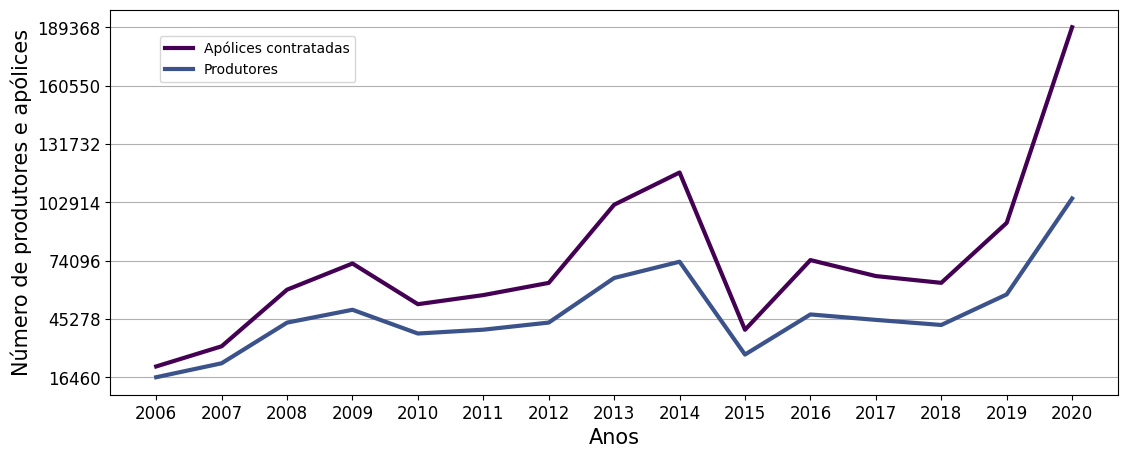
\includegraphics[width=0.6\textwidth]{img/apolices_produtores.png}
		\caption{Número de produtores e apólices de seguro rural contratadas. Brasil $2006 - 2020$}
		\small \textsuperscript {Fonte: Elaboração própria a partir de dados do Ministério da Agricultura, Pecuária e Abastecimento e da Plataforma Atlas do Seguro Rural}
	\end{figure}
\end{frame}

\begin{frame}{Artigo 1 -- Resultados}
	\begin{figure}[H]
	\centering
	\footnotesize
	
	\subfloat[Valores do prêmio e de subvenção ao prêmio\label{soma_ano_values}]{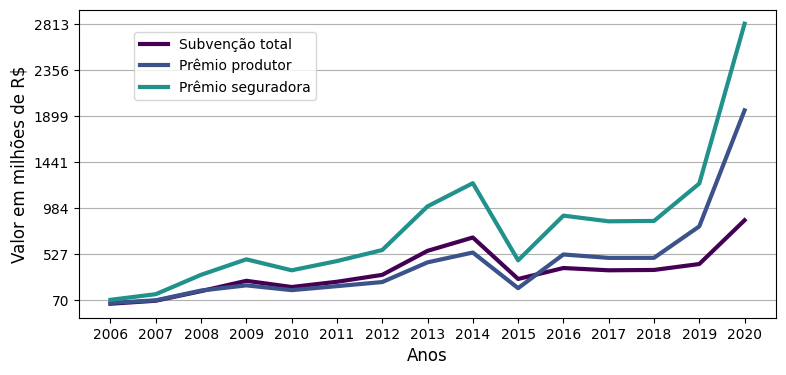
\includegraphics[width=0.3\textwidth]{img/soma_ano_values.png}}\hspace{0.1cm}
	\subfloat[Soma da importância segurada\label{total_segurado_mil}]{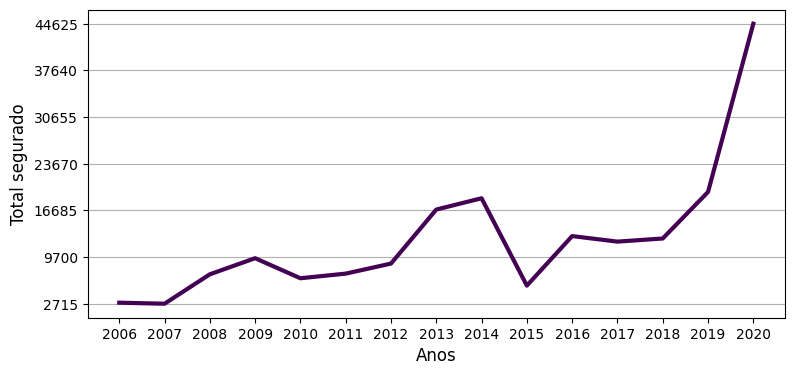
\includegraphics[width=0.3\textwidth]{img/total_segurado_mil.png}}\hspace{0.1cm}
	\subfloat[Total da área segurada em hectares.\label{area_segurada}]{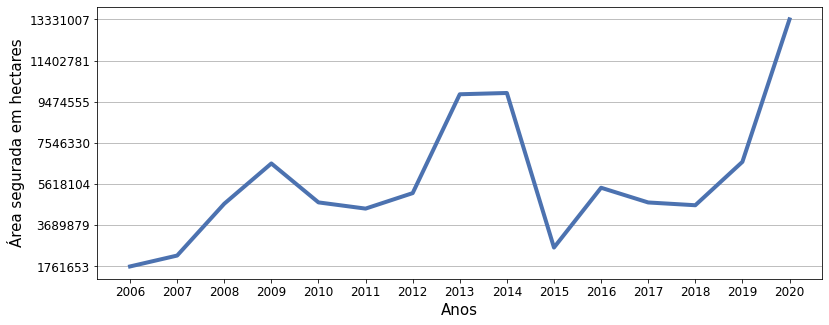
\includegraphics[width=0.3\textwidth]{img/area_segurada.png}}\\
	
	\subfloat[Número de apólices de seguro rural indenizadas\label{apolices_indenizadas}]{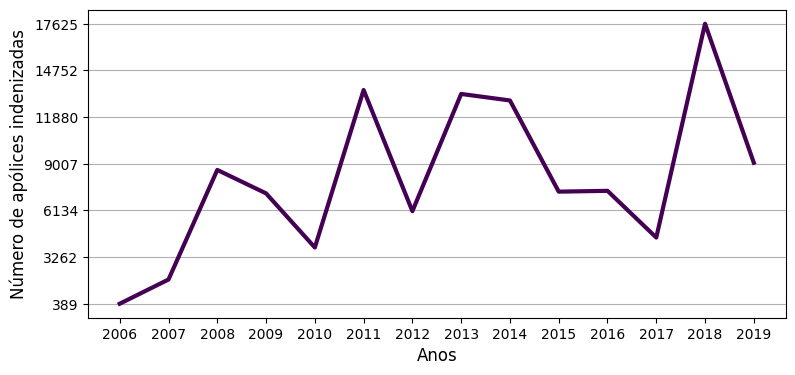
\includegraphics[width=0.3\textwidth]{img/apolices_indenizadas.png}} \hspace{0.1cm}
	\subfloat[Valor das indenizações de seguro rural pagas\label{valor_indenizacoes}]{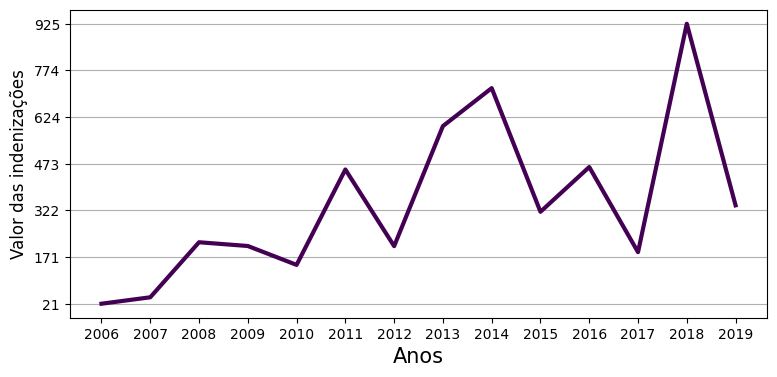
\includegraphics[width=0.3\textwidth]{img/valor_indenizacoes.png}}\hspace{0.1cm}
	\subfloat[Taxa média anual de contratação do prêmio\label{taxa_media}]{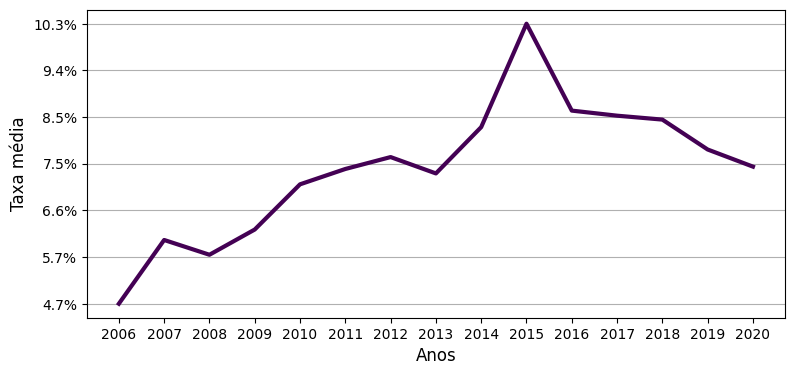
\includegraphics[width=0.3\textwidth]{img/taxa_media.png}}
	
	\caption{\footnotesize Evolução das variáveis de seguro rural no Brasil Brasil $2006 - 2019$}\label{variaveis_br}\\[-1.9ex]
	\textsuperscript{Fonte: Elaboração própria a partir de dados do Ministério da Agricultura, Pecuária e Abastecimento e da Plataforma Atlas do Seguro Rural}
\end{figure}
\end{frame}

\begin{frame}{Artigo 1 -- Resultados -- O seguro rural no Brasil}
	\begin{figure}
		\centering
		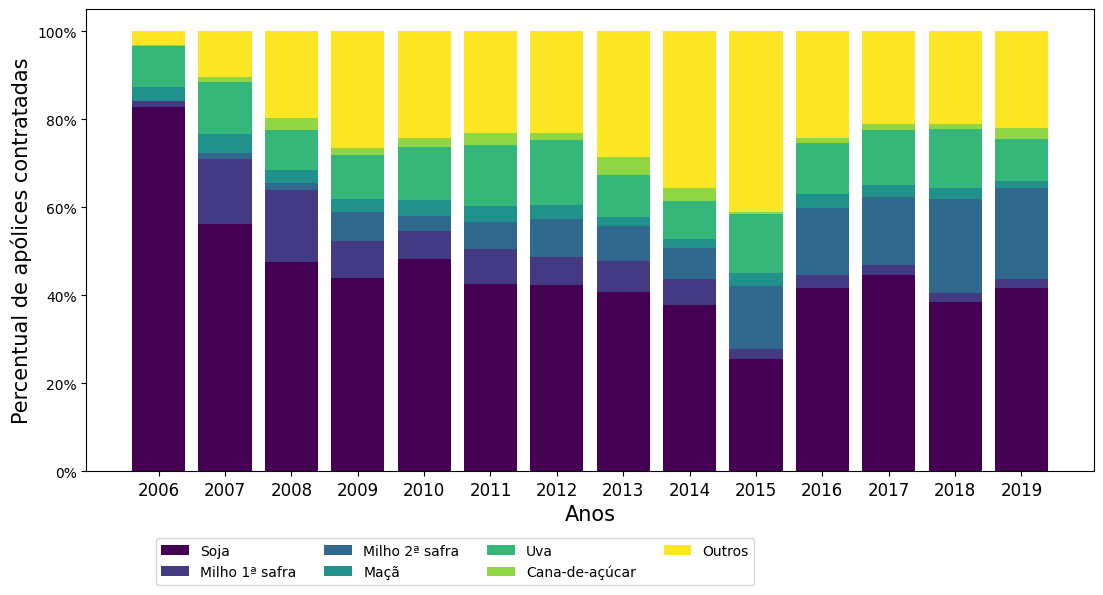
\includegraphics[width=0.6\textwidth]{img/percent_apolic_cult.png}
		\caption{Percentual da participação das maiores culturas no número de apólices de seguro rural contratadas. Brasil $2006 - 2019$}
		\small \textsuperscript {Fonte: Elaboração própria a partir de dados do Ministério da Agricultura, Pecuária e Abastecimento}
	\end{figure}
\end{frame}

\begin{frame}{Artigo 1 -- Resultados}
	\begin{figure}[H]
	\centering
	\footnotesize
	
	\subfloat[Número de apólices contratadas\label{ap_contrat_regioes}]{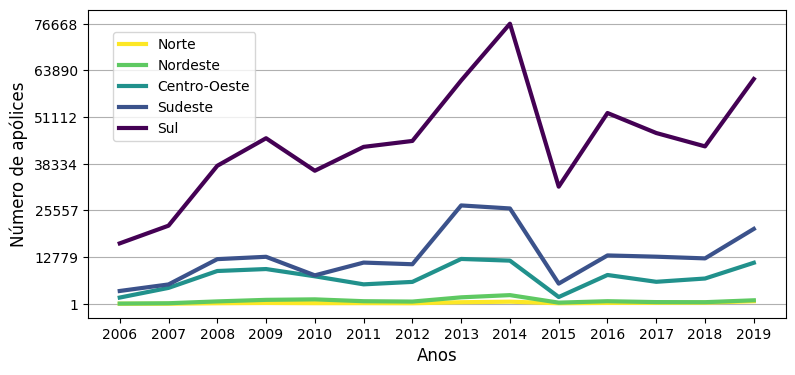
\includegraphics[width=0.3\textwidth]{img/ap_contrat_regioes.png}}\hspace{0.1cm}
	\subfloat[Total segurado (em milhões de R\$)\label{t_segurado_regioes}]{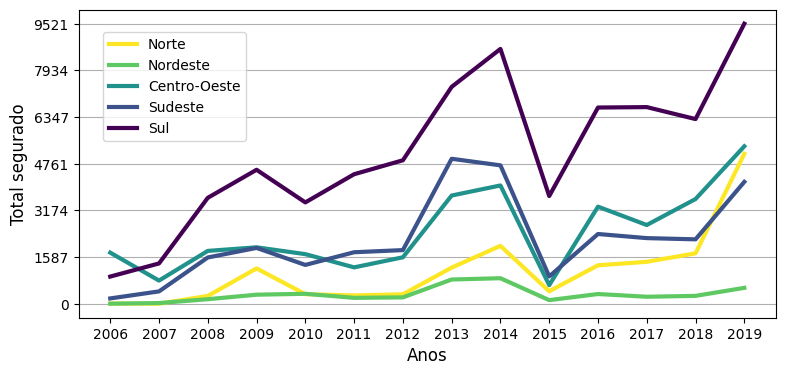
\includegraphics[width=0.3\textwidth]{img/t_segurado_regioes.png}}\hspace{0.1cm}
	\subfloat[Valores de prêmio (em milhões de R\$)\label{soma_premio_regioes}]{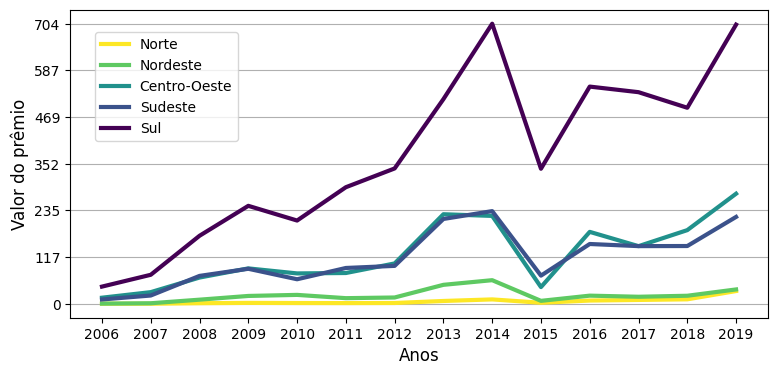
\includegraphics[width=0.3\textwidth]{img/soma_premio_regioes.png}}\\
	
	\subfloat[Valores subvenção (em milhões de R\$)\label{t_subvencao_regioes}]{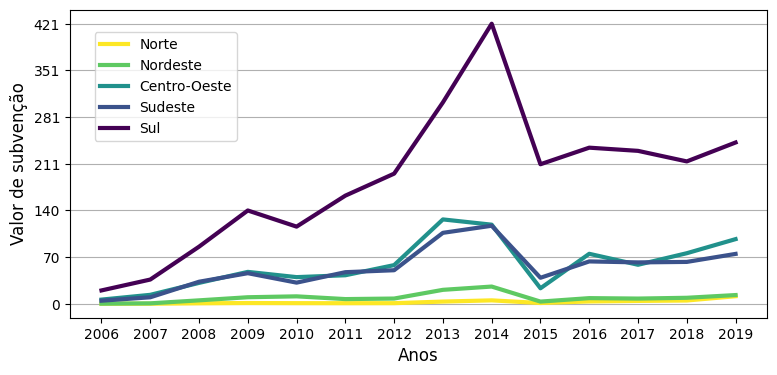
\includegraphics[width=0.3\textwidth]{img/t_subvencao_regioes.png}}\hspace{0.1cm}
	\subfloat[Apólices indenizadas\label{ap_indeniz_regioes}]{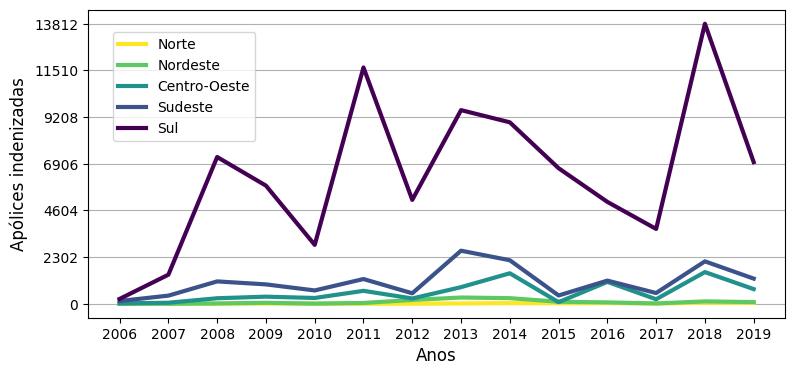
\includegraphics[width=0.3\textwidth]{img/ap_indeniz_regioes.png}}\hspace{0.1cm}
	\subfloat[Valor das indenizações (em milhões de R\$)\label{inde_pagas_regioes}]{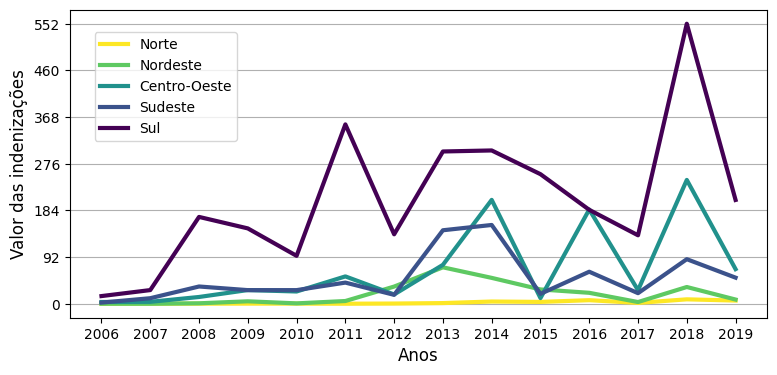
\includegraphics[width=0.3\textwidth]{img/inde_pagas_regioes.png}}\\
	
	\caption{\footnotesize Evolução das variáveis de seguro rural por regiões. Brasil $2006 - 2019$.}\label{variaveis_br}\\[-1.9ex]
	\textsuperscript{Fonte: Elaboração própria a partir de dados do Ministério da Agricultura, Pecuária e Abastecimento e da Plataforma Atlas do Seguro Rural}
\end{figure}
\end{frame}

\begin{frame}{Artigo 1 -- Resultados  -- Distribuição espacial}
	\begin{figure}
		\centering
		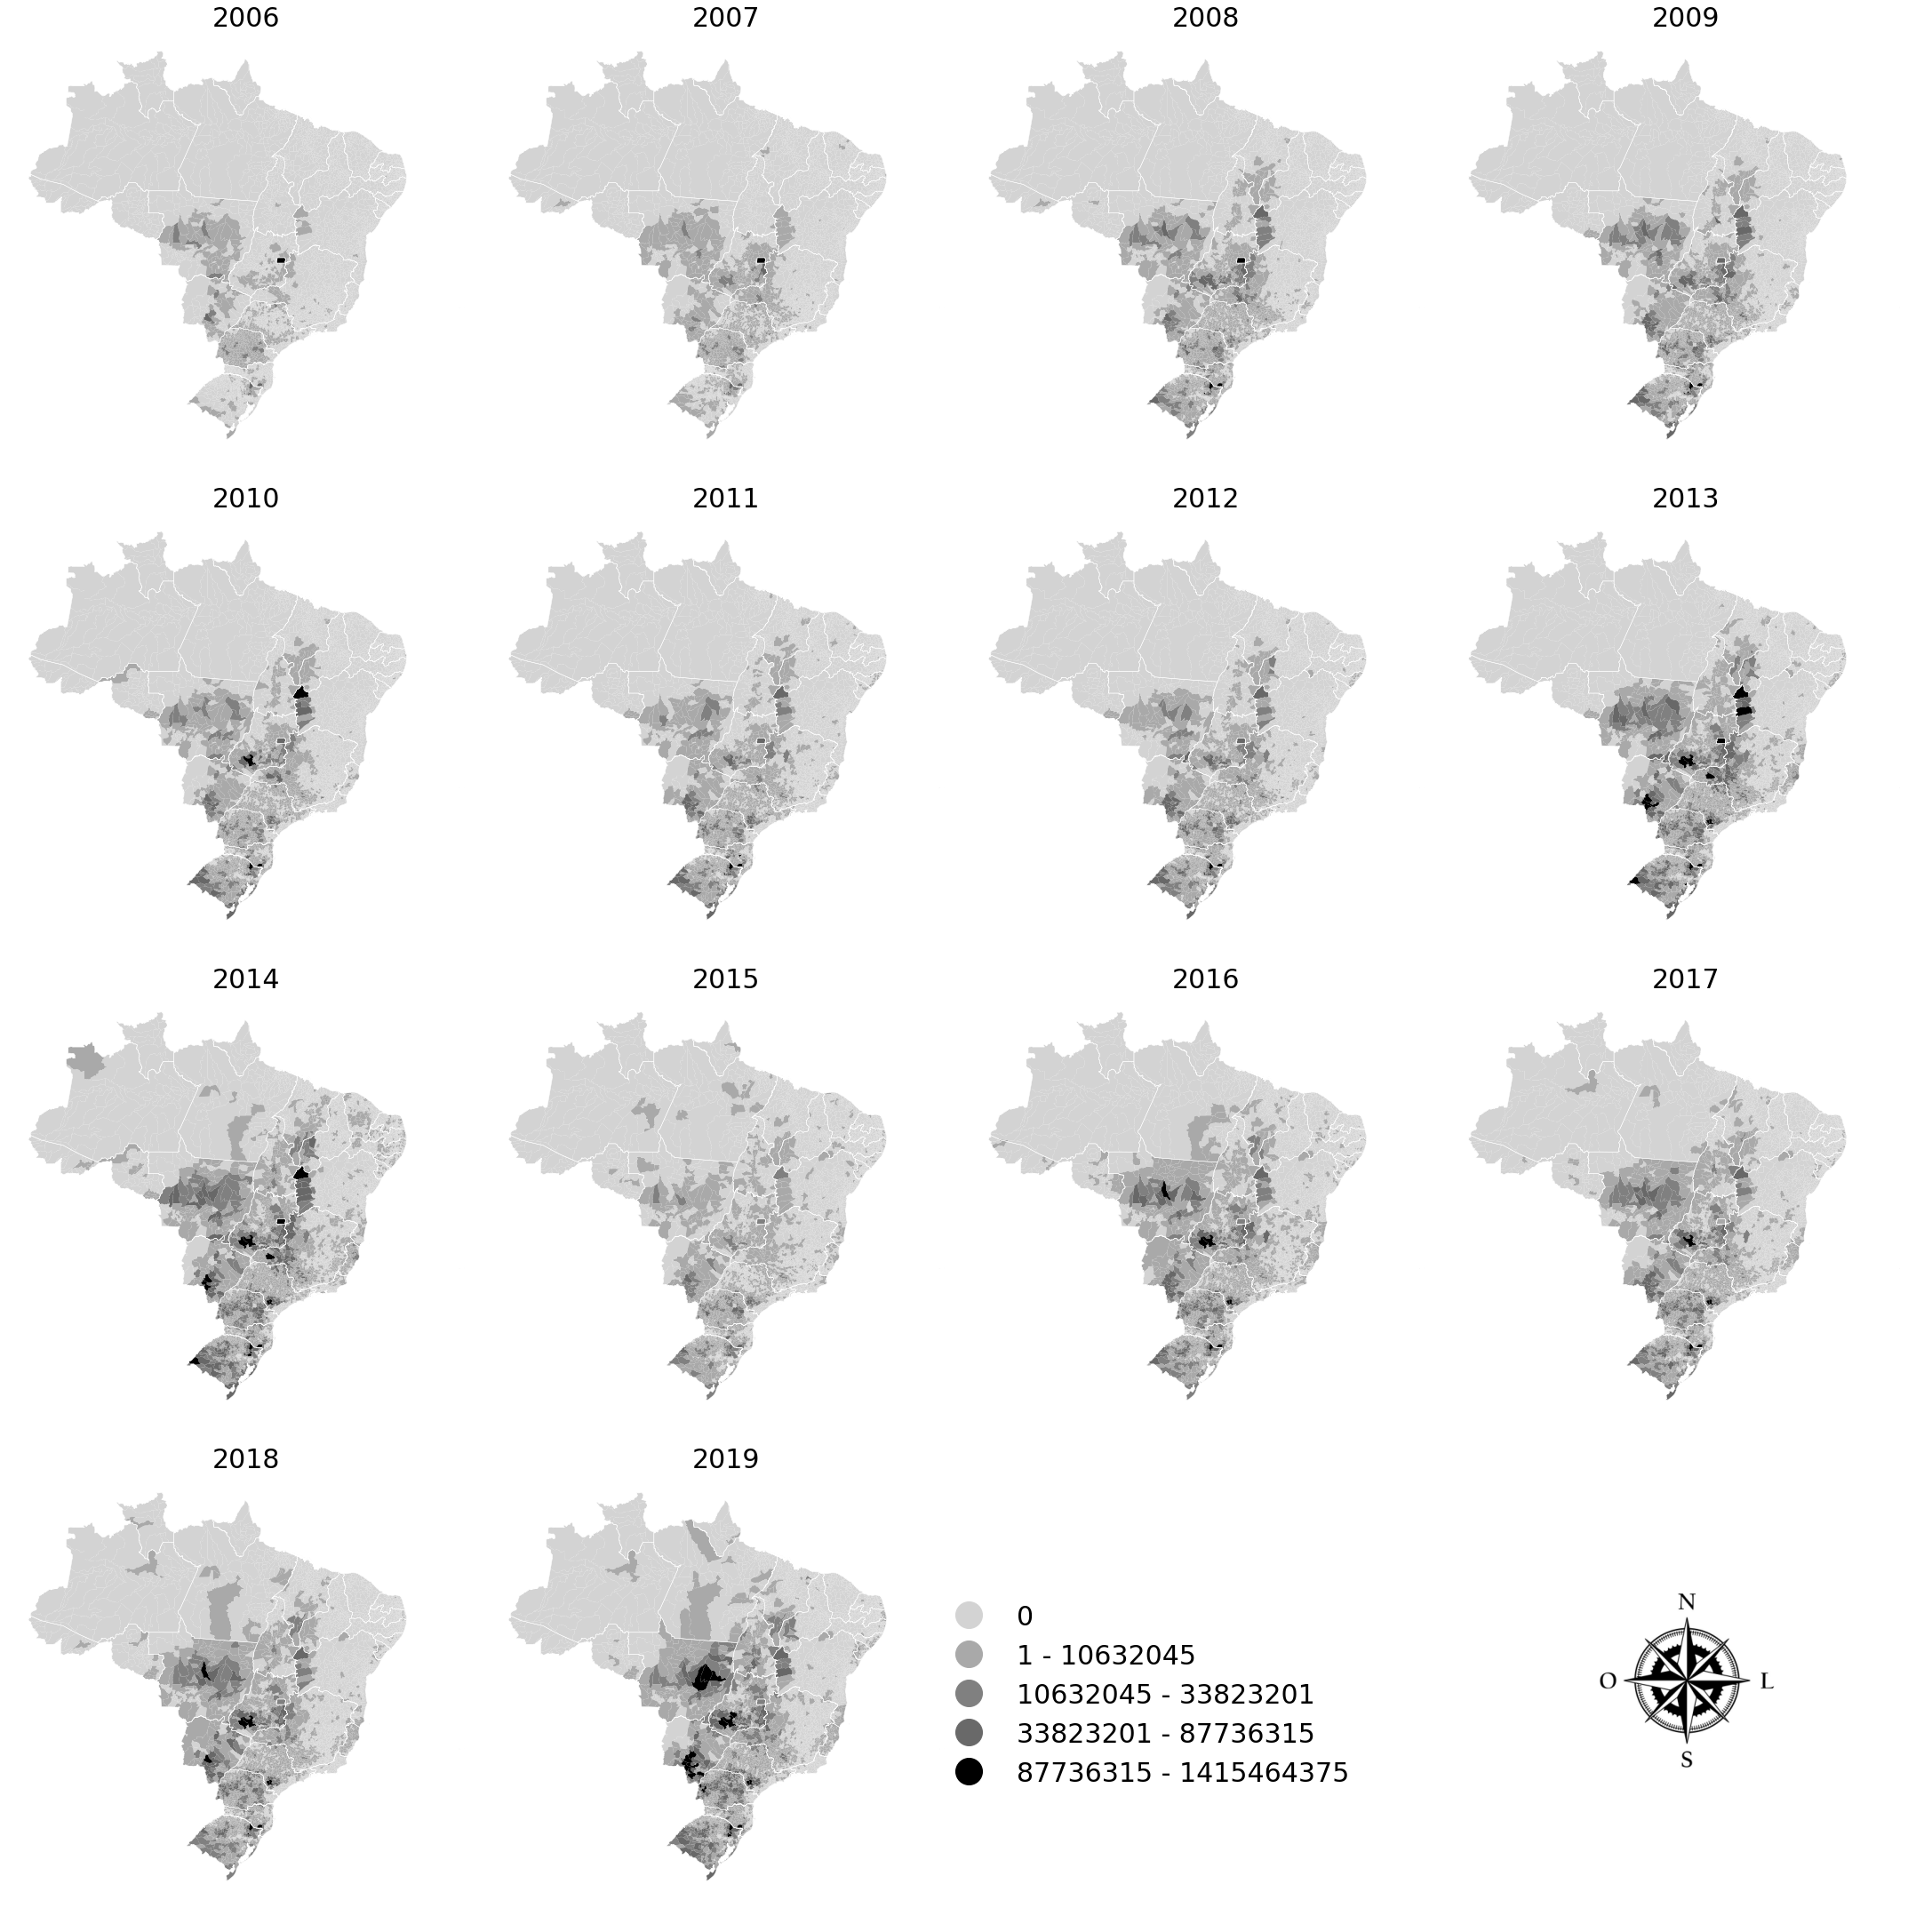
\includegraphics[width=0.4\textwidth]{img/map_total_segurado_mil.png}
		\caption{Total segurado por municípios (em mil R\$). Brasil $2006 - 2019$.}
		\small \textsuperscript {Fonte: Elaboração própria.}
	\end{figure}
\end{frame}

\begin{frame}{Artigo 1 -- Resultados  -- Distribuição espacial}
	\begin{figure}
		\centering
		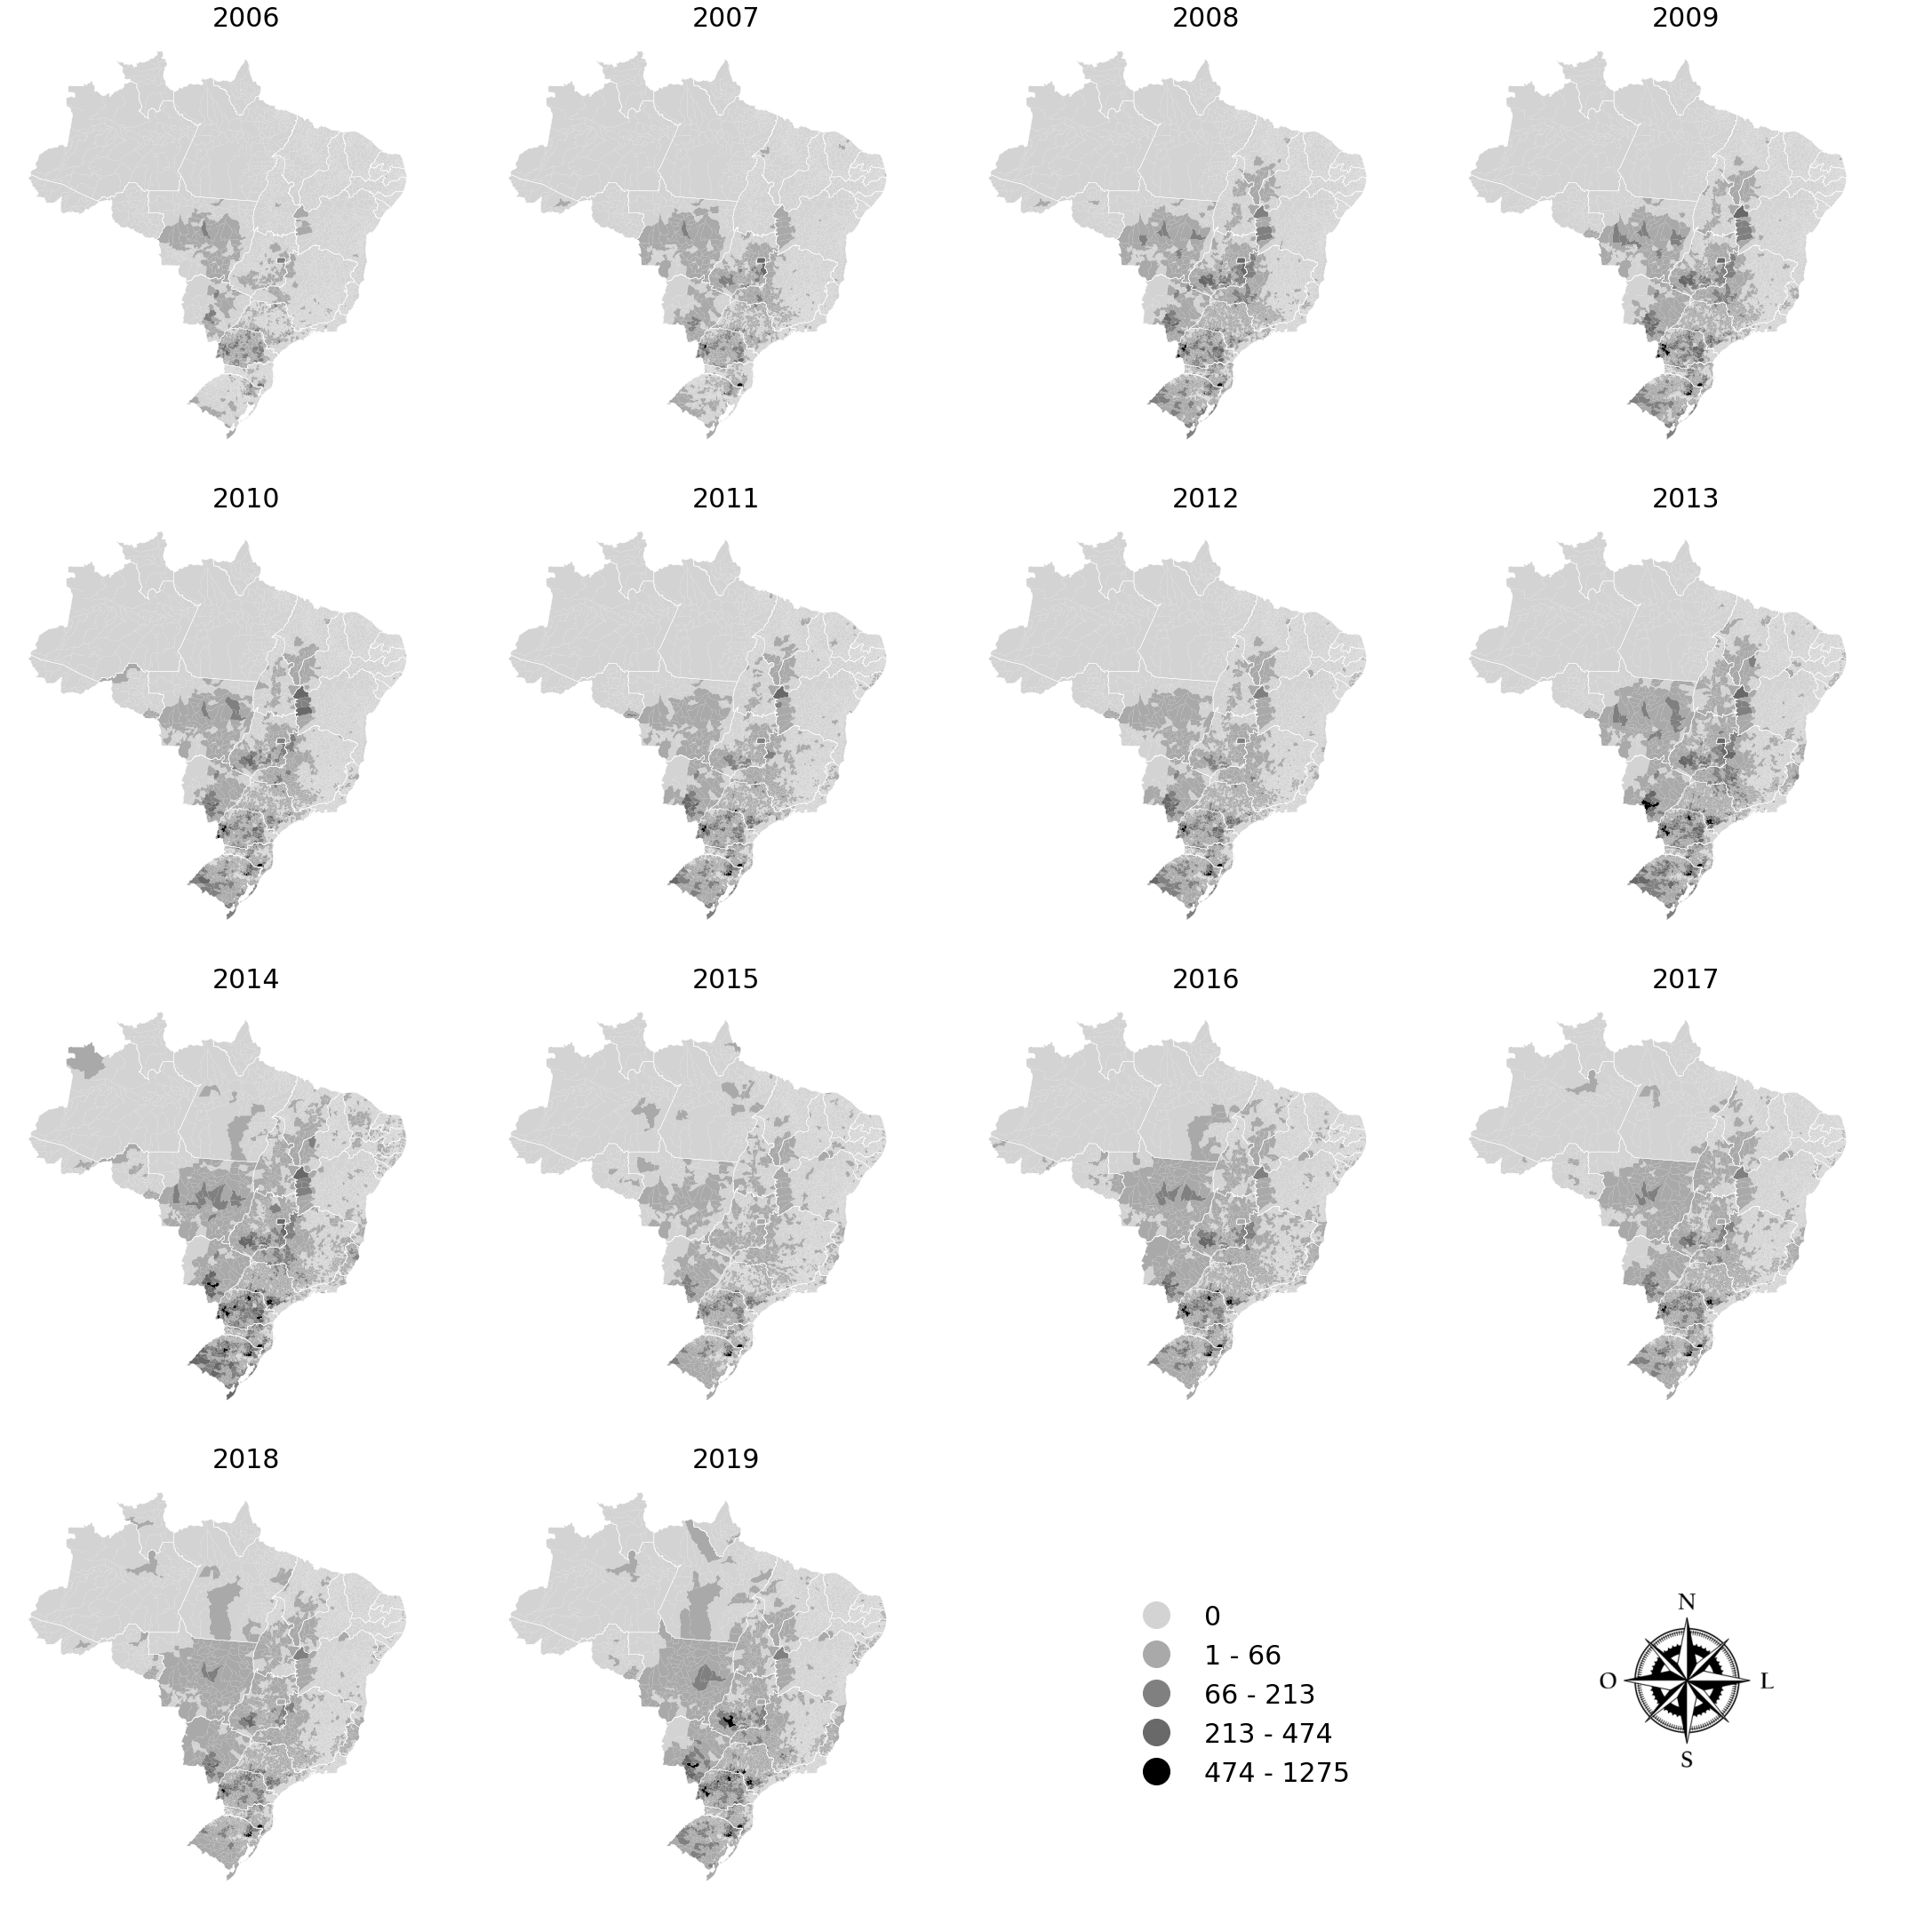
\includegraphics[width=0.4\textwidth]{img/map_apolices_contratadas.png}
		\caption{Número de apólices de seguro rural contratadas por municípios. Brasil $2006 - 2019$.}
		\small \textsuperscript {Fonte: Elaboração própria.}
	\end{figure}
\end{frame}

\subsection{Considerações finais}

\begin{frame}{Artigo 1 -- Considerações finais}
	\begin{enumerate}
	    \item Crescimento do Seguro Rural nos períodos de $2006$ a $2014$ e $2015$ a $2019$.
    	\vspace{0.25cm}
		\item Maiores concentrações apólices de Seguro Rural estão situadas nas regiões  Sul, Centro-Oeste e Sudeste, no sul do Estado de São Paulo.
	\end{enumerate}
\end{frame}

\section{Artigo 2}

\begin{frame}
\begin{alertblock}{}
    \begin{center}
        \vspace{0.1cm}
        \Large Análise de autocorrelação espacial de dados \\
        multivariados de seguro rural
        \vspace{0.1cm}
    \end{center}
\end{alertblock}
\end{frame}
\subsection{Objetivos}

\begin{frame}{Artigo 2 -- Objetivos} 
	\begin{exampleblock}{Objetivo geral}
	   \begin{itemize}
		    \item Analisar a distribuição espacial de dados multivariados do seguro rural nos municípios brasileiros entre os anos de 2006 e 2019
	    \end{itemize}
	\end{exampleblock}
	\vspace{0.5cm}
	\begin{exampleblock}{Artigo 2 -- Objetivos específicos}
	   \begin{itemize}
		    \item Investigar a presença de padrões de distribuição espacial nos dados
		    \item Avaliar a existência de dependência ou heterogeneidade espacial
	    \end{itemize}
	\end{exampleblock}
\end{frame}

\subsection{Análise de componentes principais}

\begin{frame}{Artigo 2 -- Análise de componentes principais}
    A análise de componentes principais (ACP) tem como objetivo a explicação da estrutura de covariâncias das $p$ variáveis, 
    \begin{block}{}
        $$\boldsymbol{X}^T = [X_1 \quad X_2 \quad \dots \quad X_p],$$ 
    \end{block}
    \noindent por meio de combinações lineares das variáveis originais. Os componentes principais são as $p$ combinações lineares obtidas, 
    \begin{block}{}
        $$\boldsymbol{Y}^T = [Y_1 \quad Y_2 \quad \dots \quad Y_p],$$ 
    \end{block}
    \noindent e não são correlacionados entre si.
\end{frame}

%\begin{frame}{Artigo 2 -- Análise de componentes principais}
%    O primeiro componente principal $Y_1$ é a combinação linear
%    \begin{block}{}
%	    $$Y_1 = a_{11}X_1 + a_{12}X_2 + \dots + a_{1p}X_p,$$
%    \end{block}
%	
%    \noindent cuja variância amostral é a maior dentre todas as outras combinações lineares.
%    
%    O vetor de coeficientes referente ao $j$-ésimo CP é representado por 
%    $$\boldsymbol{a}_j= [a_{j1} \quad a_{j2} \quad \dots \quad a_{jp}].$$ 
%    
%    É importante usar uma restrição nos valores desses coeficientes, geralmente
%    
%    \begin{block}{}
%        $$\boldsymbol{a}_1^T\boldsymbol{a}_1 = 1,$$ 
%    \end{block}
%    \noindent ou seja, a soma dos quadrados desses valores deve ser igual a $1$. 
%\end{frame}

%\begin{frame}{Artigo 2 -- Análise de componentes principais}
%    O segundo componente principal, $Y_2$ definido como a combinação linear
%    \begin{block}{}
%        \begin{align*}
%        	Y_2 = a_{21}X_1 + a_{22}X_2 + \dots + a_{2p}X_p,
%        \end{align*}
%    \end{block}
%    ou seja, $Y_2 = \boldsymbol{a}_2^T\boldsymbol{X}$, em que $\boldsymbol{a}_2^T = [a_{21} \quad a_{22} \quad \dots \quad a_{2p}]$ e $\boldsymbol{X}^T = [X_{1} \quad X_{2} \quad \dots \quad X_{p}]$, que possui a maior variância sujeito às condições
%    \begin{block}{}
%        \begin{align*}
%        	\boldsymbol{a}_2^T\boldsymbol{a}_2 = 1,\\
%        	\boldsymbol{a}_2^T\boldsymbol{a}_1 = 0,
%        \end{align*}
%        em que a segunda condição garante que $Y_1$ e $Y_2$ são não correlacionados. Todos os componentes são obtidos de forma similar.
%    \end{block}
%\end{frame}

\begin{frame}{Artigo 2 -- Análise de componentes principais}
    A proporção da variância total de $\boldsymbol{X}$ explicada pelo $j$-ésimo componente principal é definida por
    \begin{block}{}
        \begin{align*}
	        \dfrac{Var(Y_j)}{\textrm{Variância total de } X} = \dfrac{\lambda_j}{\textrm{traço}(\boldsymbol{S})} = \dfrac{\lambda_j}{\displaystyle\sum_{i=1}^{p}\lambda_i}.
        \end{align*}
    \end{block}
\end{frame}

\begin{frame}{Artigo 2 -- Análise de componentes principais}
    De acordo com Everitt e Hothorn (2011), os primeiros $k$ componentes, em que $k < p$, explicam uma proporção da variância total,
    \begin{block}{}
        \begin{align*}
            \dfrac{\displaystyle\sum_{j=1}^{k}Var(Y_j)}{\textrm{Variância total de } X} = \dfrac{\displaystyle\sum_{j=1}^{k}\lambda_j}{\textrm{traço}(\boldsymbol{S})} = \dfrac{\displaystyle\sum_{j=1}^{k}\lambda_j}{\displaystyle\sum_{j=1}^{p}\lambda_j}.
        \end{align*}    
    \end{block}
\end{frame}

\begin{frame}{Artigo 2 -- Análise de componentes principais}
    \begin{itemize}
        \item Os componentes principais podem ser obtidos a partir da matriz de covariâncias amostrais $\boldsymbol{S}$ ou a partir da matriz de correlações amostrais $\boldsymbol{R}$;
        \vspace{0.5cm}
        \item Extrair os componentes como os autovetores de $\boldsymbol{R}$ é equivalente a calcular os componentes das variáveis originais para depois padronizar cada um para ter variância igual a $1$.
    \end{itemize}
\end{frame}

\subsection{Análise espacial}

\begin{frame}{Artigo 2 -- Efeitos espaciais}
	\begin{itemize}
		\item \textbf{Dependência espacial}
		\vspace{0.25cm}
		\begin{itemize}
		    \item As unidades de corte transversal -- domicílios, municípios, regiões -- não são independentes entre si.
		    \item O valor de uma variável numa região $i$, $y_i$, depende do valor dessa mesma variável nas regiões vizinhas $j$, $y_j$. 
		\end{itemize}
		\item \textbf{Heterogeneidade espacial}
		\vspace{0.25cm}
		\begin{itemize}
			\item Ocorre quando há instabilidade estrutural através das regiões $\rightarrow$ diferentes respostas dependendo da localidade.
		\end{itemize}
	\end{itemize}
\end{frame}

\begin{frame}{Artigo 2 -- Matriz de ponderação espacial}
	\begin{itemize}
	    \item É uma medida de proximidade entre as regiões.
	    \item Para um conjunto de $n$ áreas é definida como: 
	    \begin{align*}
        	\boldsymbol{W} =
	        \left[
	        \begin{array}{cccc}
		        w_{11} & w_{12} & \dots & w_{1n} \\
		        w_{21} & w_{22} & \dots &w_{2n} \\
		        \vdots & \vdots & \ddots & \vdots \\
		        w_{n1} & w_{n2} & \dots & w_{nn}\\
	        \end{array}
	        \right],
        \end{align*}
        \noindent Cada elemento $w_{ij}$ representa uma medida de proximidade entre as áreas $i$ e $j$. 
        \[
            w_{ij} = 
            \begin{cases}
                \text{1,} & \quad\text{se $i$ e $j$ são contíguos} \\
                \text{0,} & \quad\text{se $i$ e $j$ não são contíguos.}\\
            \end{cases}
        \]
        \noindent Por convenção, $w_{ij}=0,\quad \forall i=j$
	\end{itemize}
\end{frame}

%\begin{frame}{Operador de defasagem espacial}
%    \begin{itemize}
%        \item \textbf{Defasagem}
%    \end{itemize}
%    $$y_{ij} \rightarrow y_{i-1,j},\text{ } y_{i,j-1},\text{ } y_{i+1,j},\dots$$  
%    \begin{block}{}
%        $$ \boldsymbol{W} \times y = Wy $$    
%    \noindent em que $\boldsymbol{W}$ é a matriz de pesos espaciais, $y$ é o vetor da variável e $Wy$ é a defasagem espacial da variável
%    \end{block}
%    \begin{itemize}
%        \item $Wy$ é a média do valor da variável nas regiões vizinhas se a matriz de pesos for normalizada nas linhas.
%    \end{itemize}
%\end{frame}

\begin{frame}{Artigo 2 -- Autocorrelação espacial global}
	\begin{itemize}
		\item Um índice de autocorrelação espacial mede a associação espacial nos dados considerando o \textbf{local} e o \textbf{valor} da variável em estudo.
		\item Hipótese: Aleatoriedade na distribuição espacial da variável. 
	\end{itemize}
	
	\begin{figure}
		\centering
		\small
		\subfloat[Positiva\label{fig:a}]{
\includegraphics[width=0.15\textwidth]{img/autocor_pos.png}}\hspace{0.2cm}
		\subfloat[Nula\label{fig:b}]{
\includegraphics[width=0.15\textwidth]{img/autocor_null.png}}\hspace{0.2cm}
		\subfloat[Negativa\label{fig:c}]{
\includegraphics[width=0.15\textwidth]{img/autocor_neg.png}}
		\caption{Padrões de autocorrelação espacial}
		\small \textsuperscript {Fonte: Radil (2011)}
		\label{padroes_autocorr}
	\end{figure}
	\begin{itemize}
		\item É necessário usar uma estatística de teste para a aleatoriedade da distribuição espacial global da variável.
	\end{itemize}
\end{frame}

\begin{frame}{Artigo 2 -- \textit{I} de Moran}
	O \textit{I} de Moran mede a relação do desvio padronizado de uma variável $z$ numa área $i$ com o desvio padronizado das 	áreas vizinhas $j$ para a mesma variável $z$ (ALMEIDA, 2012).
	
	\begin{block}{}
		\small
		\begin{align}
		\label{IMoran}
		I = \dfrac{n}{S_0} \dfrac{\displaystyle\sum_{i} \sum_{j} w_{ij} z_i z_j}{\displaystyle\sum_{i=1}^{n} z_i^2}.
		\end{align}
		\noindent \small em que $z_i = (x_i - \bar{x})$, $w_{ij}$ é uma medida de contiguidade entre $i$ e $j$,  $n$ é o número de regiões e $S_0$ é a soma dos pesos espaciais ($w_{ij}$)
	\end{block}	
\end{frame}

\begin{frame}{Artigo 2 -- Autocorrelação espacial local}
	\begin{itemize}
		\item Estatísticas globais fornecem padrões de associação espacial em todo o conjunto de dados
		\item Medidas de autocorrelação local buscam identificar padrões no interior de uma região de estudo  
		\item Podem informar a existência de um \textit{cluster} de valores autocorrelacionados em nível local
		\item Podem informar sobre existência de \textit{outliers} locais
		\item Para Anselin (1995), um indicador local de associação espacial (\textit{LISA}) deve satisfazer a dois critérios:
		\vspace{0.25cm}
		\begin{enumerate}
			\item Deve indicar clusters espaciais estatisticamente significativos;
			\item A soma dos indicadores locais deve ser levar ao indicador global.
		\end{enumerate}
	\end{itemize}
\end{frame}

\begin{frame}{Artigo 2 -- \textit{I} de Moran local}
	Um indicador local de associação espacial do tipo \textit{LISA} é o \textit{I} de Moran local que é expresso por: 
	\begin{block}{}
		\small
		\vspace{0.25cm}
		\begin{align*}
		I_i = z_i \sum_{j}^{} w_{ij} z_j,
		\end{align*}
		\noindent \small em que $z_i$ e $z_j$ são os valores da variável padronizada nas regiões $i$ e $j$, $w_{ij}$ é uma matriz de pesos espaciais.
	\end{block}	
\end{frame}

\subsection{Material e métodos}

\begin{frame}{Artigo 2 -- Material e métodos -- Dados}
	Dados de apólices de seguro rural dos municípios brasileiros de 2006 a 2019. 
	\vspace{0.5cm}
    \begin{itemize}
        \item $5570$ Municípios
        \item $14$ anos
        \item $7$ variáveis
        \item \textit{Shapefile} dos municípios brasileiros. (IBGE, 2020).
        \item $373$ divergências relacionadas à distritos e outras localidades.
        \begin{itemize}
            \item Dados divergentes foram atribuídos aos municípios geograficamente mais próximos. 
        \end{itemize}
        \item  Atlas do Seguro Rural e Ministério da Agricultura, Pecuária e Abastecimento.
    \end{itemize}
\end{frame}

\begin{frame}{Artigo 2 -- Material e métodos -- Variáveis}
    \begin{center}
    \small
        \begin{tabular}{ll}
            \hline 
            Sigla & Variável  \tabularnewline
            \hline 
            Total de apólices contratadas                  & TAC       \\ % ap\_contrat   
            Soma da importância segurada (R\$ milhão)      & SIS       \\ % t\_segurado   
            Soma dos prêmios (R\$ milhão)                  & SPR       \\ % soma\_premio  
            Total de subvenção (R\$ milhão)                & TSB       \\ % t\_subvencao  
            Soma das indenizações pagas (R\$ milhão)       & SIP       \\ % inde\_pagas   
            Taxa média aplicada às apólices                & TMA       \\ % tx\_media     
            Número de apólices indenizadas                 & NAI       \\ % ap\_indeniz 
            %\tabularnewline
            \hline 
            \vspace{0.1cm}
            \footnotesize{Fonte: Elaboração própria}
            \end{tabular}
    \end{center}    
\end{frame}

\begin{frame}{Artigo 2 -- Material e métodos -- Procedimento de análise}
    \begin{enumerate}
        \item \textbf{Análise de Componentes Principais (ACP):} 
        \begin{itemize}
            \item Reduzir a dimensionalidade dos dados;
            \item Incorporar aos escores do primeiro componente principal informação das variáveis originais. 
        \end{itemize}
        \item \textbf{Análise Exploratória de Dados Espaciais (AEDE):} 
        \begin{itemize}
            \item Aplicada aos escores do primeiro componente principal, com o objetivo de investigar a presença de padrões de distribuição espacial.
        \end{itemize}
    \end{enumerate}
\end{frame}

\subsection{Resultados}

\begin{frame}{Artigo 2 -- Resultados}
	\begin{figure}
		\centering
		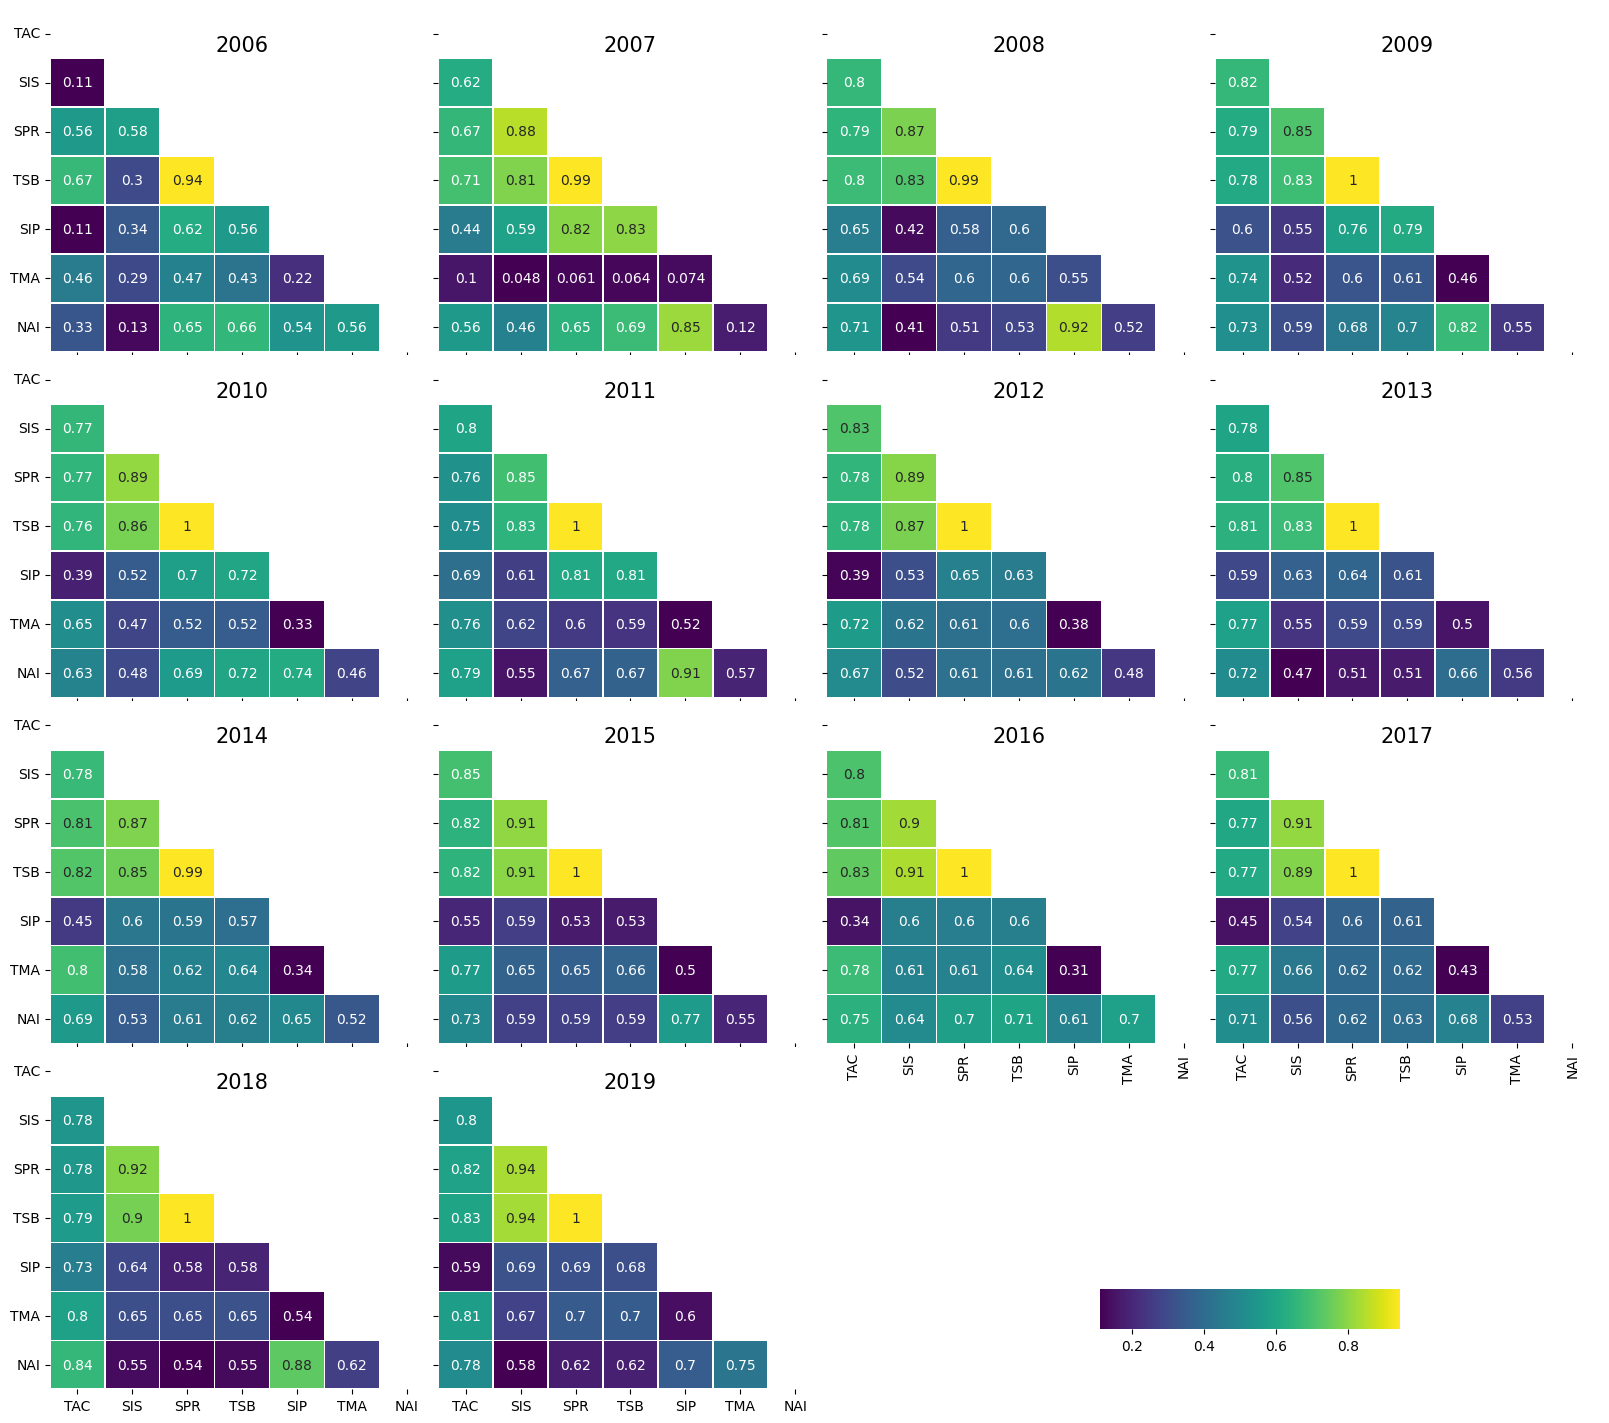
\includegraphics[width=0.46\textwidth]{img/corr_anos.png}
		\caption{Correlação entre as variáveis de seguro Rural. Brasil $2006$ -- $2019$}
		\small \textsuperscript {Fonte: Elaboração própria a partir de dados do Ministério da Agricultura, Pecuária e Abastecimento (MAPA).}
	\end{figure}
\end{frame}

\begin{frame}{Artigo 2 -- Resultados}
	\begin{figure}
		\centering
		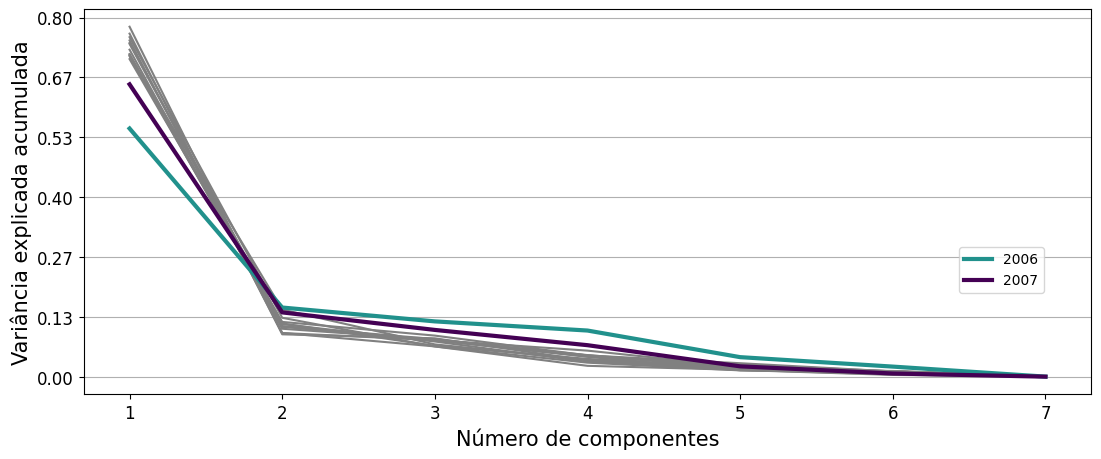
\includegraphics[width=0.7\textwidth]{img/var_radio.png}
		\caption{Variância explicada acumulada pelos componentes principais. Brasil $2006$ -- $2019$}
		\small \textsuperscript {Fonte: Elaboração própria.}
	\end{figure}
\end{frame}

\begin{frame}{Artigo 2 -- Resultados}
	\begin{figure}
		\centering
	    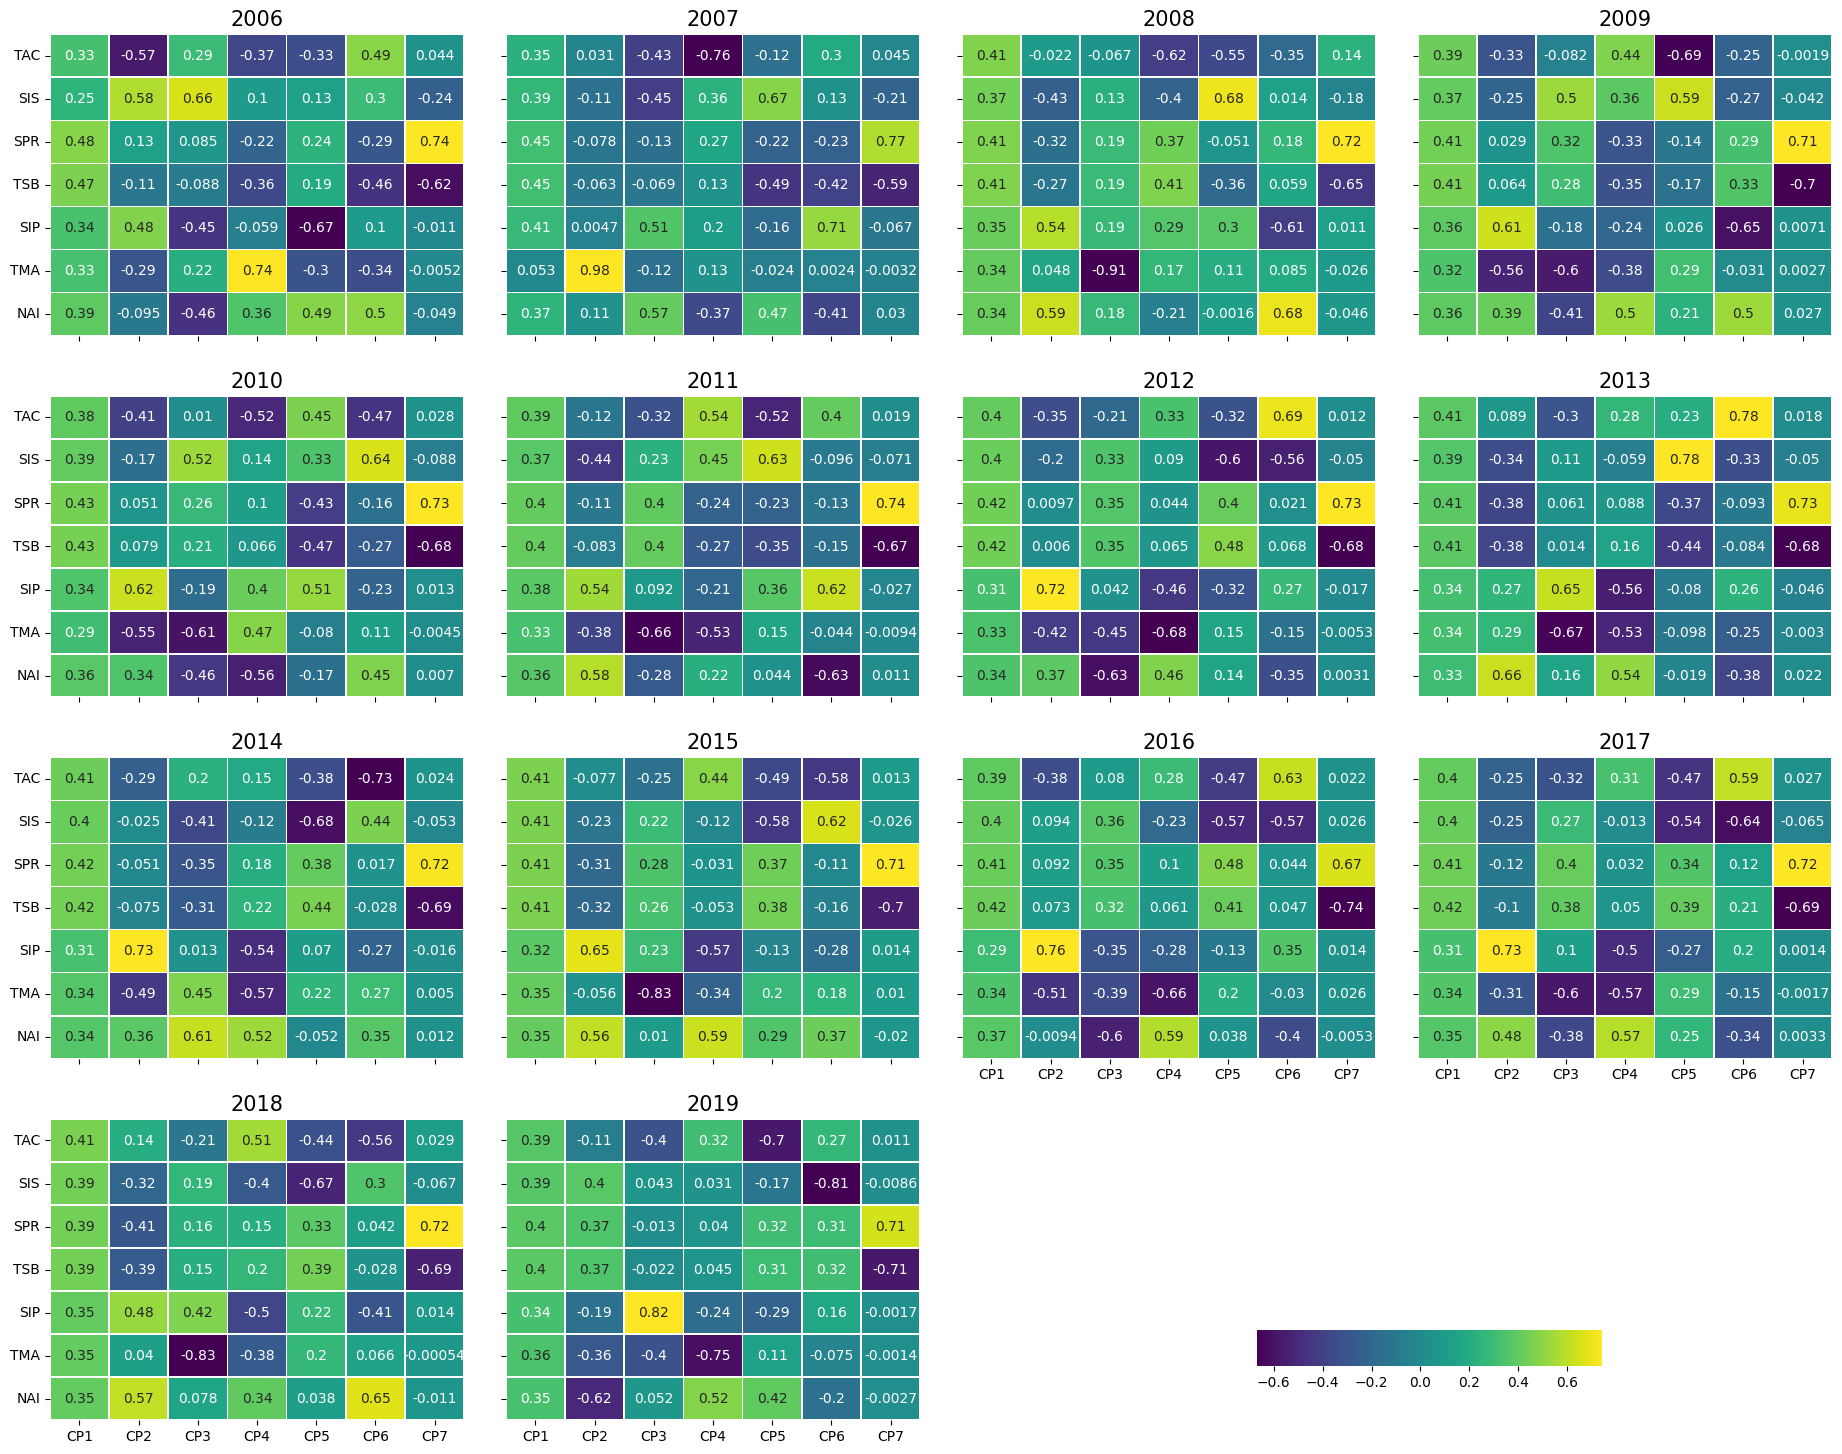
\includegraphics[width=0.5\textwidth]{img/corr_pca_var.png}
	    \caption{Correlação entre as variáveis de seguro Rural. Brasil $2006$ -- $2019$.}
		\small \textsuperscript {Fonte: Elaboração própria.}
	\end{figure}
\end{frame}

\begin{frame}{Artigo 2 -- Resultados  -- Distribuição espacial}
	\begin{figure}
		\centering
		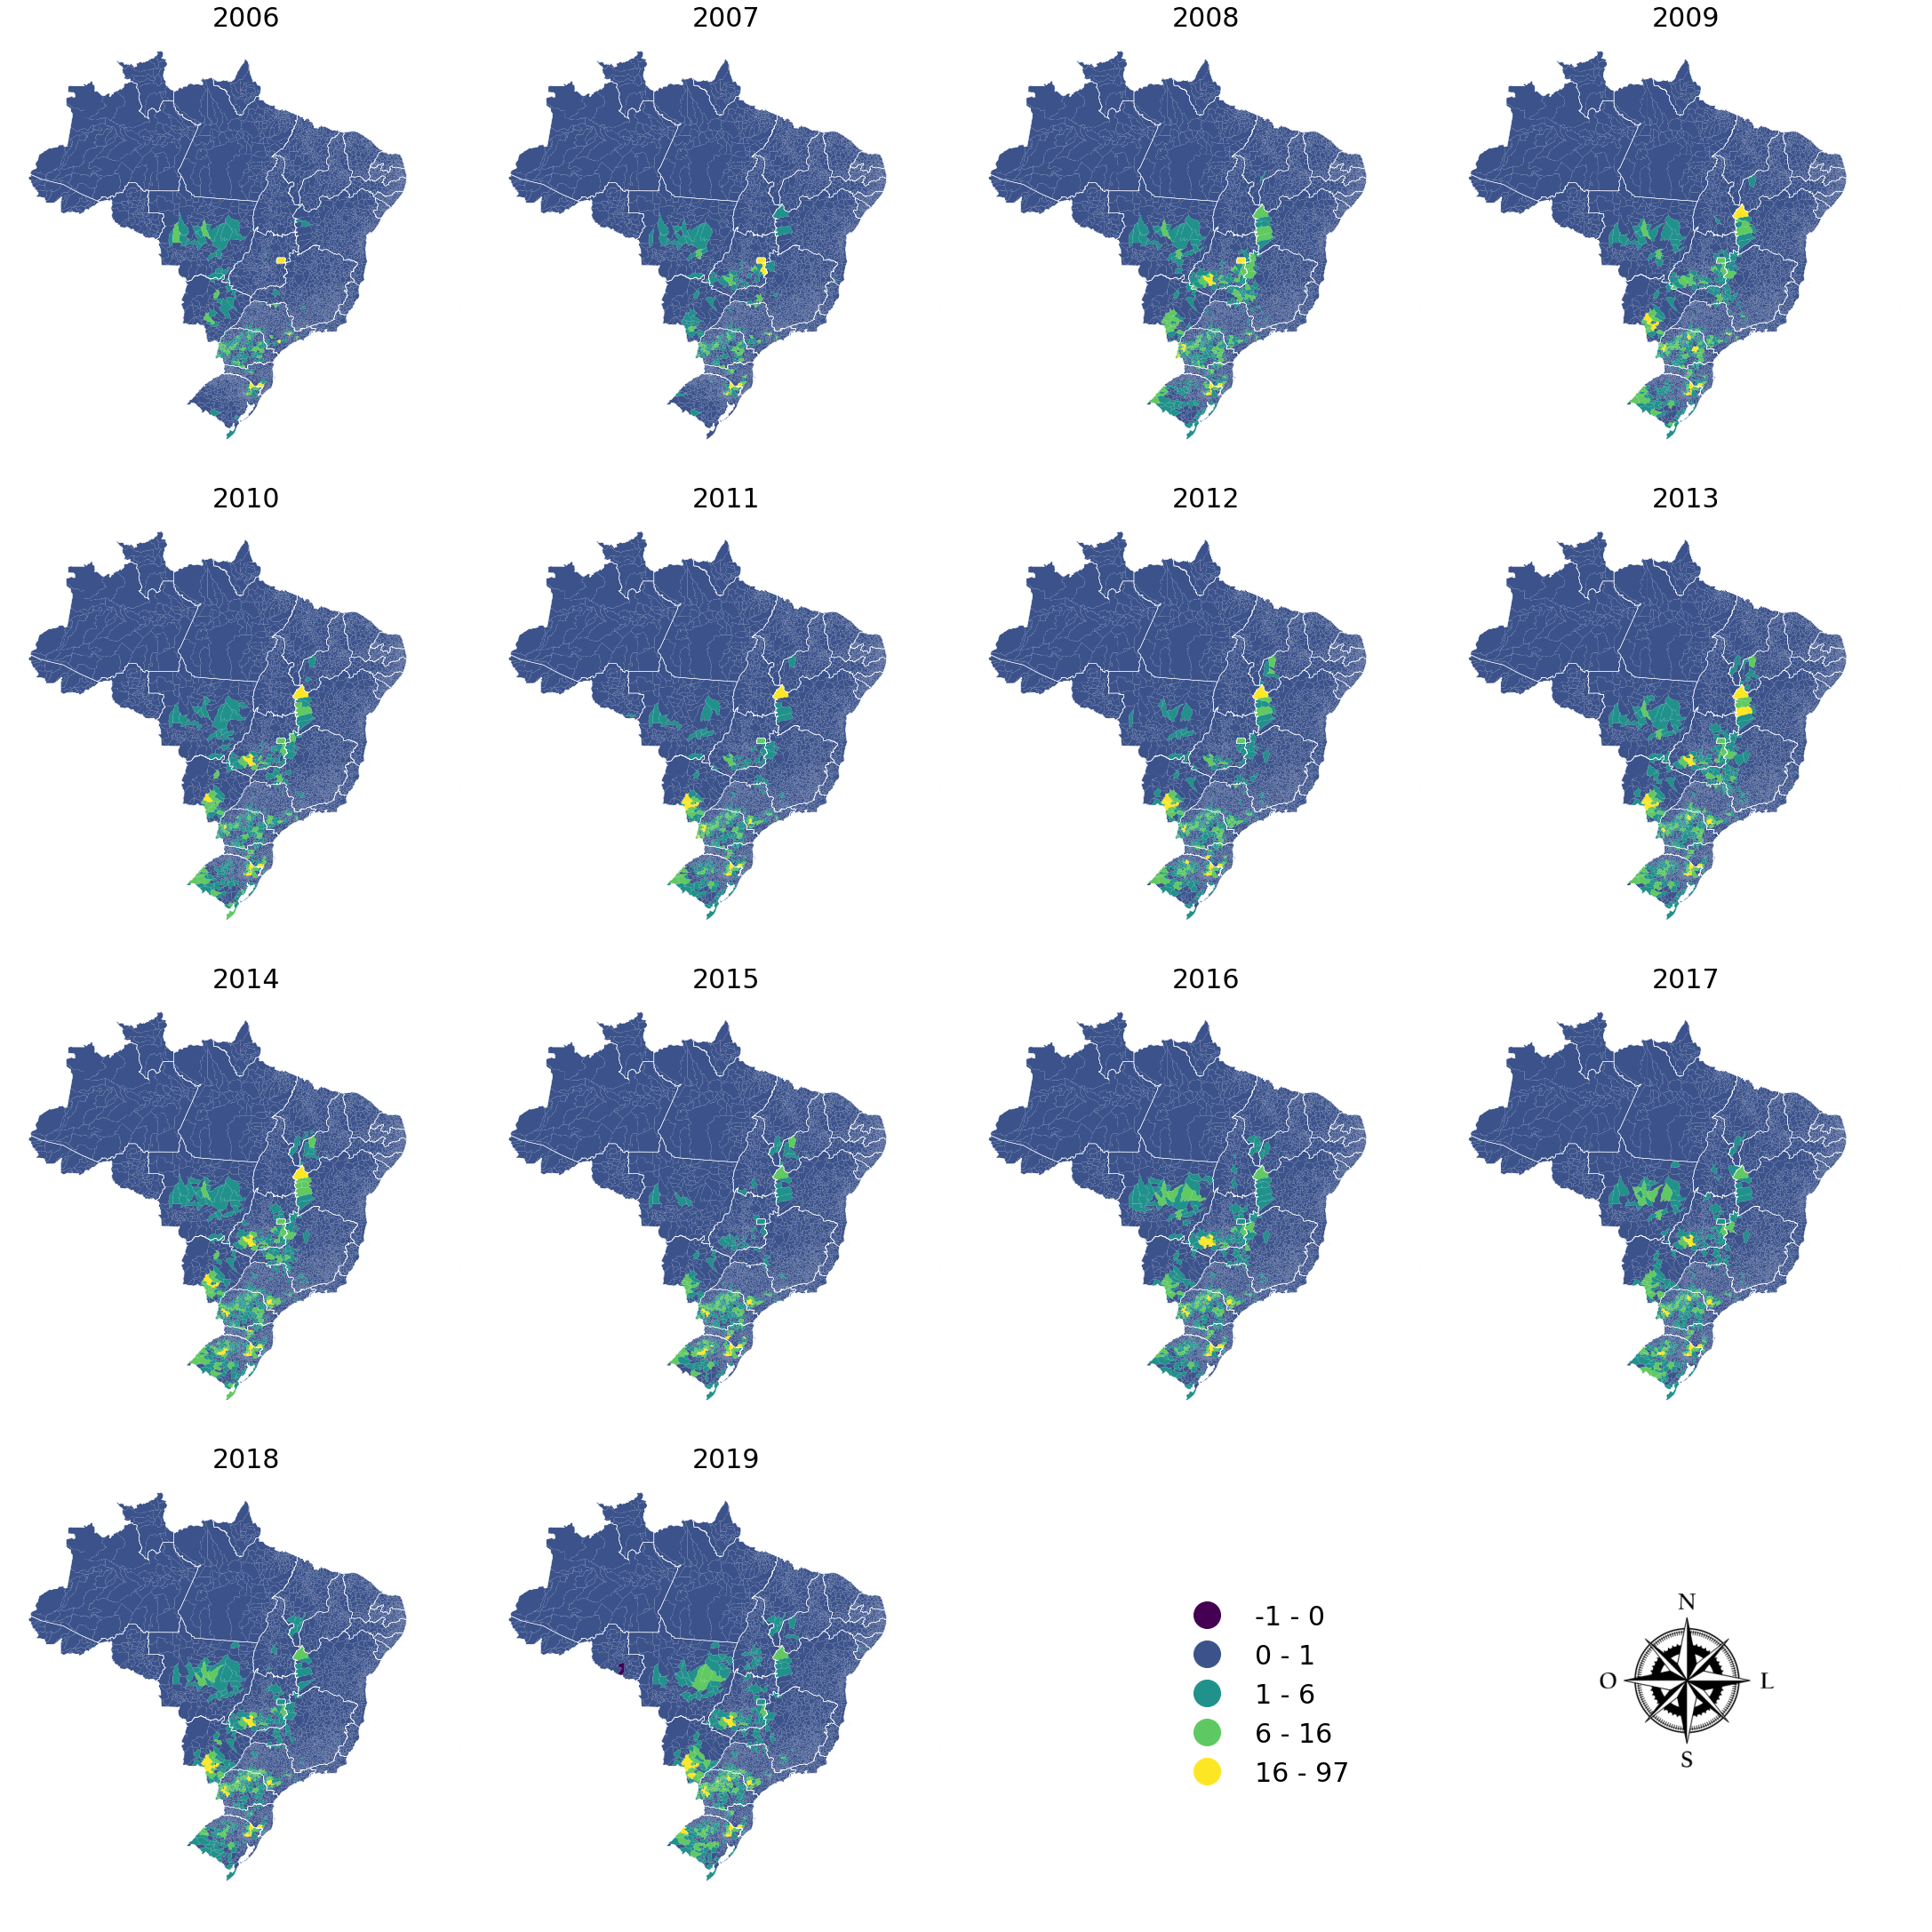
\includegraphics[width=0.43\textwidth]{img/map_CP1_color.png}
		\caption{Distribuição espacial do primeiro componente principal. Brasil $2006$ -- $2019$.}
		\small \textsuperscript {Fonte: Elaboração própria.}
	\end{figure}
\end{frame}

\begin{frame}{Artigo 2 -- Resultados -- Autocorrelação espacial (\textit{I} de Moran)}
	\begin{figure}
		\centering
	    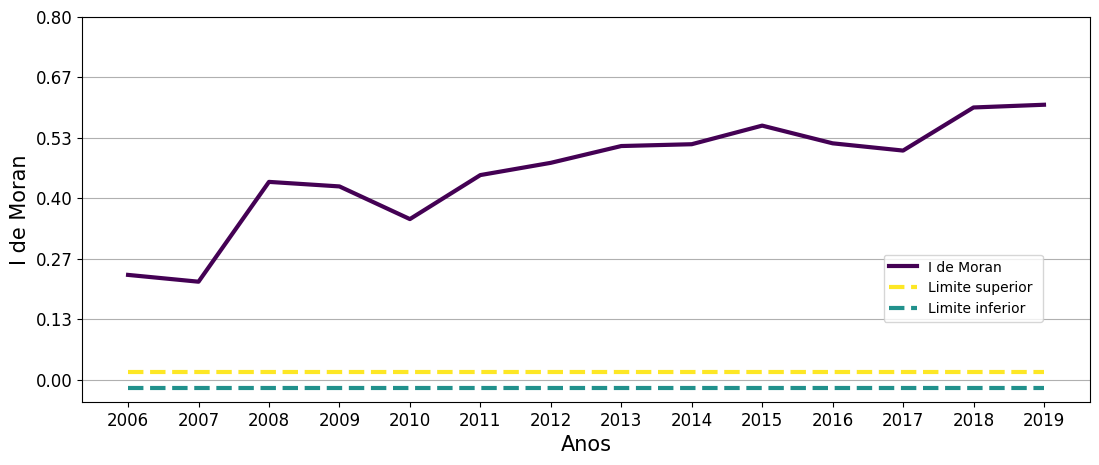
\includegraphics[width=0.6\textwidth]{img/i_de_moran_cp1.png}
	    \caption{Autocorrelação espacial (\textit{I} de Moran) do primeiro componente principal. Brasil $2006$ -- $2019$}
		\small \textsuperscript {Fonte: Elaboração própria.}
	\end{figure}
\end{frame}

\begin{frame}{Artigo 2 -- Resultados -- \textit{I} de Moran local}
	\begin{figure}
		\centering
		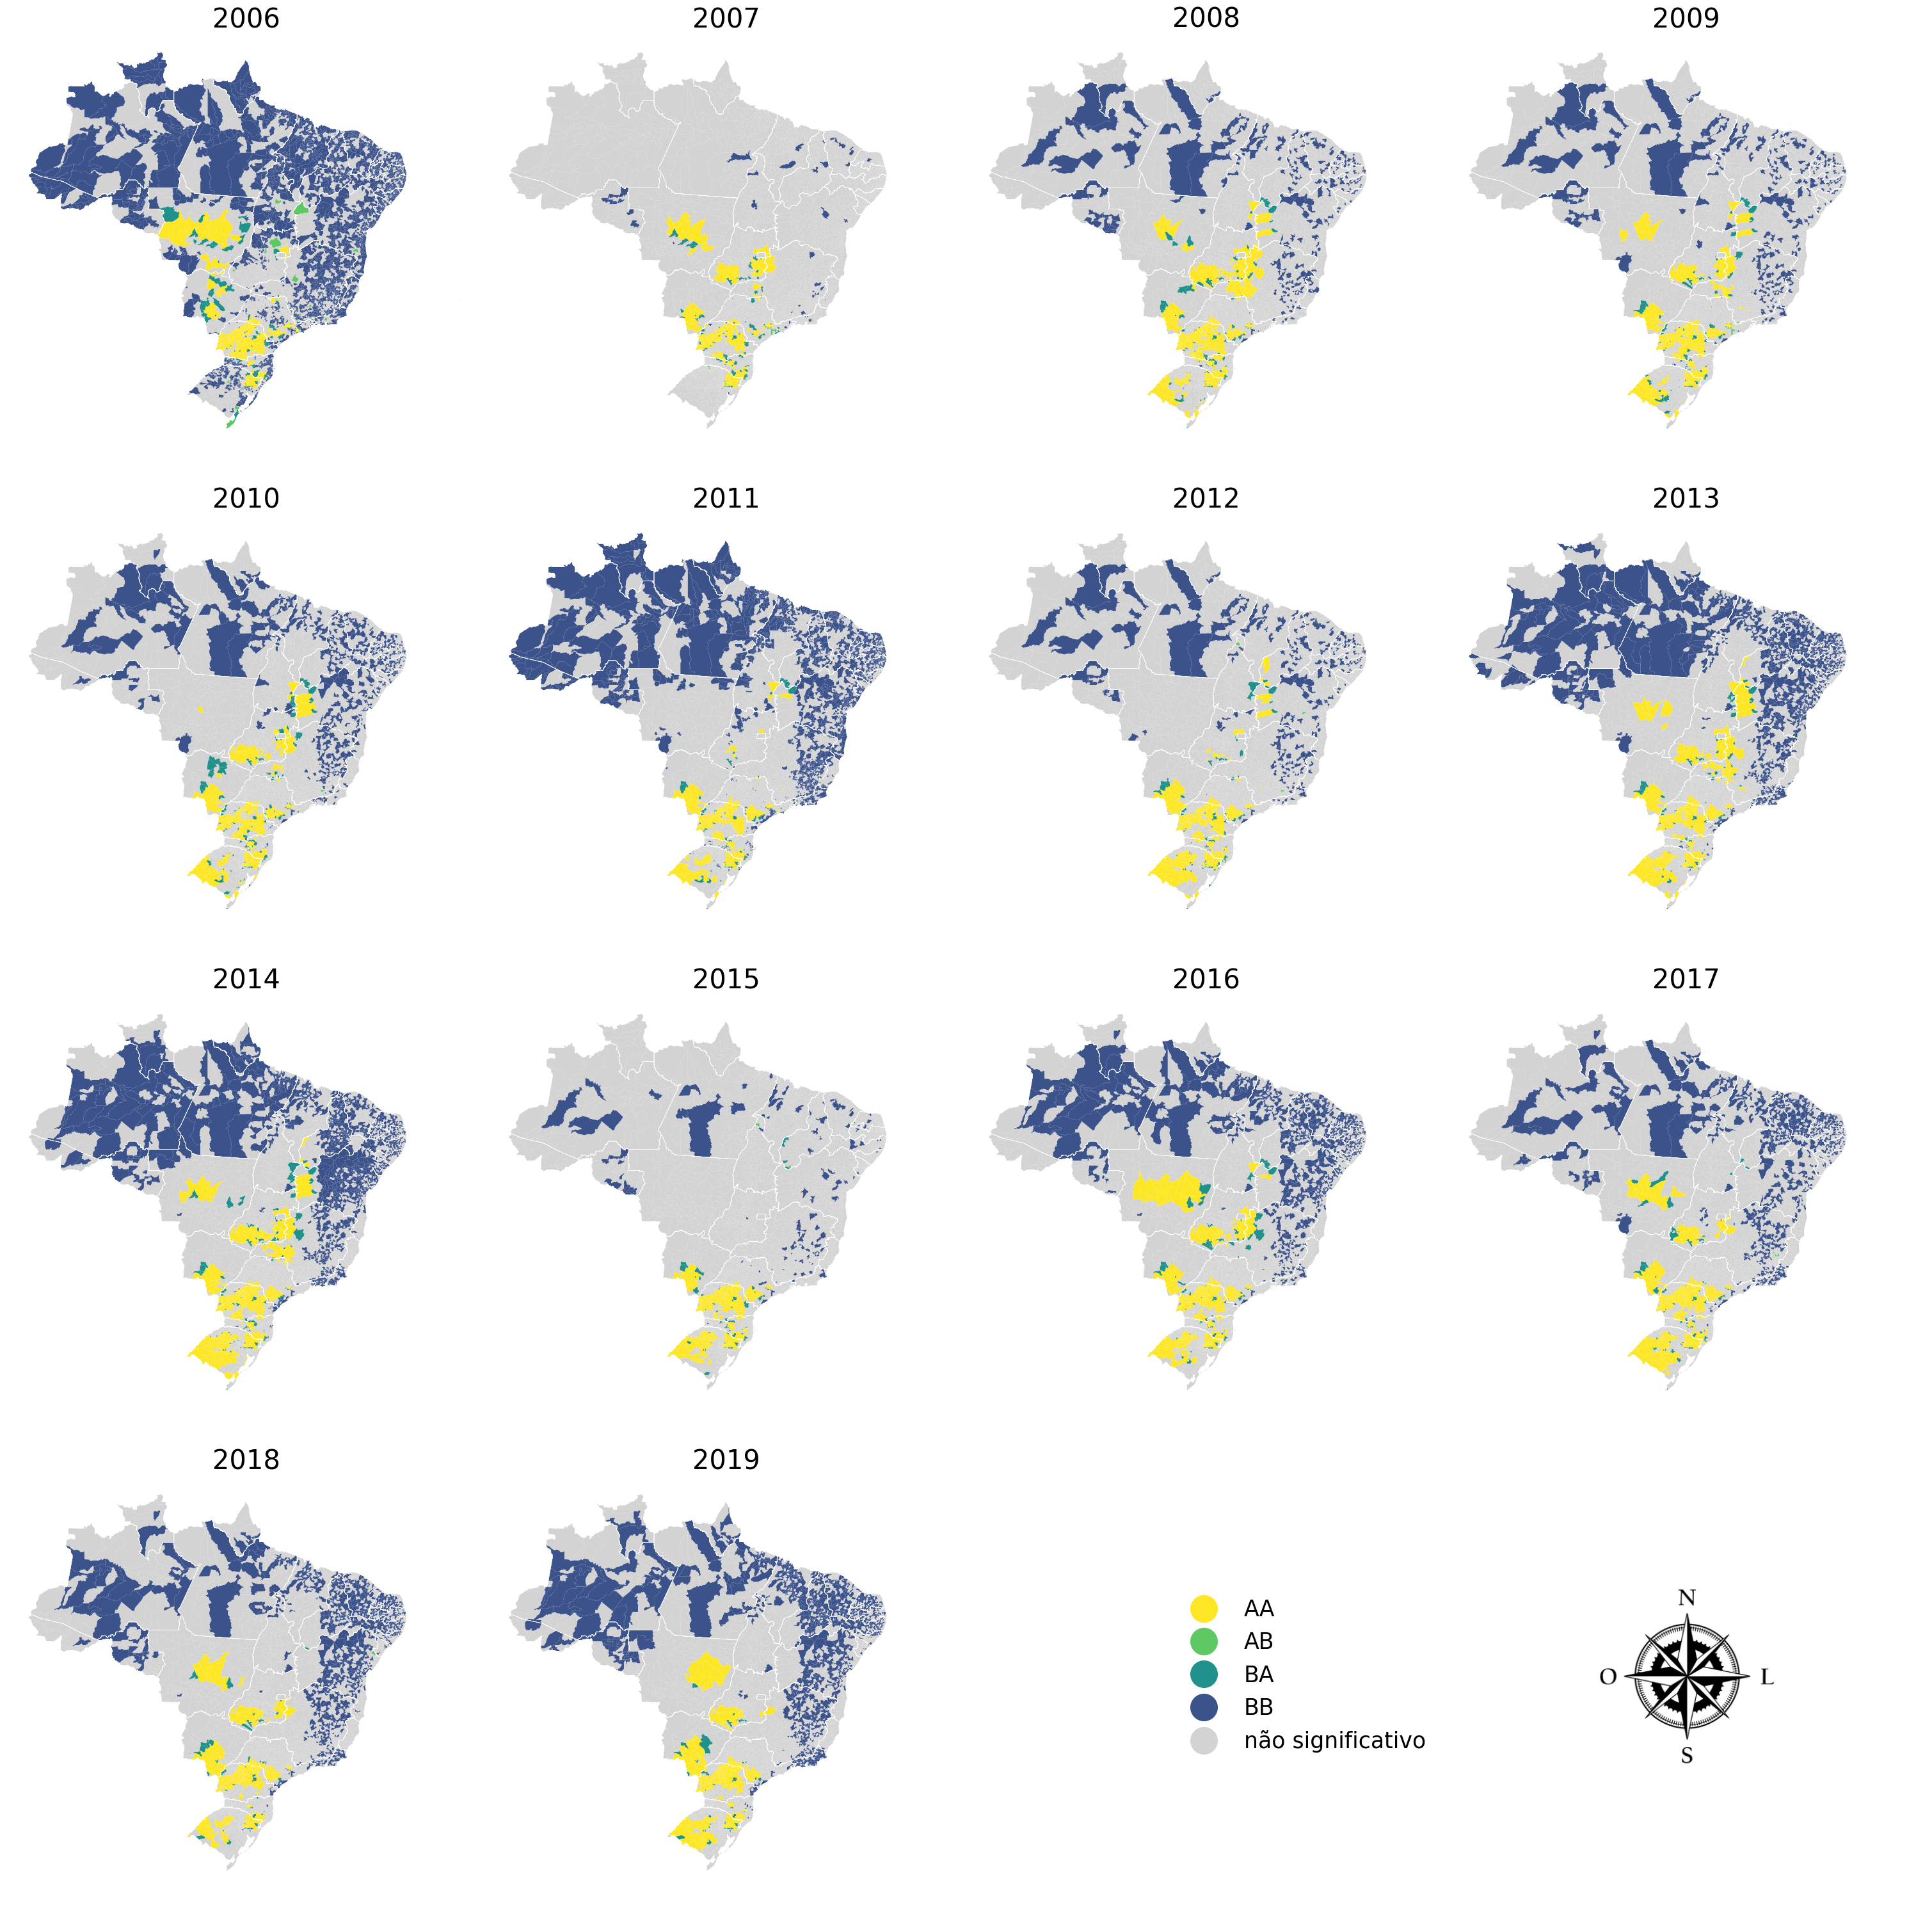
\includegraphics[width=0.43\textwidth]{img/map_lisa_cp1_viridis.png}
		\caption{Mapas \textit{LISA} para o primeiro componente principal.  Brasil $2006$ -- $2019$.}
	\end{figure}
\end{frame}

\subsection{Considerações finais}

\begin{frame}{Artigo 2 -- Considerações finais}
	\begin{enumerate}
	    \item Devido à estrutura de correlação entre as variáveis de seguro rural foi possível utilizar os escores do primeiro componente principal como uma variável representativa das variáveis originais. 
	    \vspace{0.25cm}
	    \item Os escores do primeiro componente principal positivamente correlacionados com todas as variáveis originais. 
	    \vspace{0.25cm}
	    \item As maiores concentrações do Seguro Rural estão situadas nas regiões  Sul, Centro-Oeste e Sudeste, no sul do Estado de São Paulo.
    \end{enumerate}
\end{frame}

\section{Considerações finais}

\begin{frame}{Considerações finais}
		\begin{enumerate}
	    \item Crescimento do Seguro Rural entre $2006$ e $2019$.
	    \vspace{0.25cm}
		\item Existe dependência espacial em todos os anos analisados.
		\vspace{0.25cm}
		\item Aumento na dependência espacial do Seguro Rural ao longo dos anos analisados.
		\vspace{0.25cm}
		\item Maiores concentrações apólices de Seguro Rural estão situadas nas regiões Sul, Centro-Oeste e Sudeste, no sul do Estado de São Paulo.
		\vspace{0.25cm}
		\item Foi possível utilizar os escores do primeiro componente principal como uma variável representativa das variáveis originais.
	\end{enumerate}
\end{frame}

\section{Referências}

\begin{frame}{Referências}
	\begin{flushleft}
			\footnotesize{  

				{ALMEIDA, E. \textbf{Econometria Espacial Aplicada}. Campinas-SP: Alínea, 2012.}
				
				\vspace{0.2cm}
					
				{ANSELIN, L. Local indicatos of spatial association - LISA. \textbf{Geographical analysis}, v. 27, p. 93-115, 1995.}	

				\vspace{0.2cm}
				
				{CENTRO DE ESTUDOS AVANÇADOS EM ECONOMIA APLICADA (0CEPEA) \textbf{PIB do Agronegócio Brasileiro}. Disponível em: \url{https://www.cepea.esalq.usp.br/br/pib-do-agronegocio-brasileiro.aspx}. Acesso em: 26 jun 2021.}
				
				\vspace{0.2cm}
				
				{EVERITT, B.; HOTHORN, T. \textbf{An introduction to applied multivariate analysis with R.} Nova York: Springer-Verlag, 2011.}
				
				\vspace{0.2cm}
				
                {INSTITUTO BRASILEIRO DE GEOGRAFIA E ESTATÍSTICA - IBGE. \textbf{Censo Agropecuário 2017}. Rio de Janeiro, v. 8, p.1-105, 2019.}
                
                \vspace{0.2cm}
                
                {INSTITUTO BRASILEIRO DE GEOGRAFIA E ESTATÍSTICA - IBGE. \textbf{Malha Municipal}.  Disponível em: \url{https://ibge.gov.br/geociencias/organizacao-do-territorio/estrutura-territorial/15774-malhas.html?=&t=o-que-e} Acesso em: 18 out. 2020.}

				\vspace{0.2cm}
				
		    	{REY, S. J.; ANSELIN, L. PySAL: A Python library of spatial analytical methods.\textbf{ Review of Regional Studies}, v. 37, n. 1, p. 5–27, 2007.}
		    }
	\end{flushleft}
\end{frame}

\end{document}
